%%This article template was last updated 30 September 2003 --- Tim Null
%%It is part of the
%%Pmetrika LaTeX Style File Package for Psychometrika Authors
%%This is the \LaTeX2e "article" template for the journal Psychometrika.
%%It can be freely used and modified by anyone.
%%
%% ITEM 1 [See the "howto.tex" file.]
%%
\documentclass[titlepage, a4paper, 11pt]{article}

%%ITEM 2 [See the "howto.tex" file.]
\usepackage[dvips]{graphicx}
%\usepackage[draft,dvips]{graphicx}
%\usepackage[pdftex]{graphicx}
%\usepackage[draft,pdftex]{graphicx}

%% ITEM 3 [See the "howto.tex" file.]
\usepackage[myheadings]{fullpage}
\usepackage{pmetrika}
\usepackage{float}
\usepackage{csquotes}
\usepackage{hyperref}

\usepackage[natbibapa]{apacite}
\bibliographystyle{apacite}
\usepackage{etoolbox}
\renewenvironment{APACrefURL}[1][]{}{}
\AtBeginEnvironment{APACrefURL}{\renewcommand{\url}[1]{}}
\renewcommand{\doiprefix}{doi:~\kern-1pt}
\renewcommand{\APACrefnote}[1]{}

\usepackage{amsfonts}
\usepackage{amsmath}
\usepackage{submit}
\usepackage{svg}
\usepackage{makecell}

%% ITEM 4 [See the "howto.tex" file.]
%\setcounter{secnumdepth}{3}


%% ITEM 5 [See the "howto.tex" file.]
%%%%%%%%%%%%%%%%%%%%%%%%%%%%%%%%%%%%%%%%%%%%%%%%%%%%%%%
%%   ENTER YOUR PERSONAL PREAMBLE ITEMS IN THIS SECTION
%%             Some examples provided
%%%%%%%%%%%%%%%%%%%%%%%%%%%%%%%%%%%%%%%%%%%%%%%%%%%%%%%
%%  Begin Section  %%%%%%%%%%%%%%%%%%%%%%%%%%%%%%%%%%%%
%%%%%%%%%%%%%%%%%%%%%%%%%%%%%%%%%%%%%%%%%%%%%%%%%%%%%%%
%\usepackage{}
%\usepackage{}
%input
\def\diag{\mathrm{diag}}
\def\vec{\mathrm{vec}}
\def\cov{\mathrm{cov}}
\def\tr{\mathrm{Tr}}
\def\pr{\mathrm{Pr}}
\AtBeginDocument{\renewcommand{\APACrefYearMonthDay}[3]{\BBOP{#1}\BBCP}}
%%%%%%%%%%%%%%%%%%%%%%%%%%%%%%%%%%%%%%%%%%%%%%%%%%%%%%%
%%  End Section  %%%%%%%%%%%%%%%%%%%%%%%%%%%%%%%%%%%%%%
%%%%%%%%%%%%%%%%%%%%%%%%%%%%%%%%%%%%%%%%%%%%%%%%%%%%%%%



\begin{document}

%% ITEM 6 [See the "howto.tex" file.]
\begin{titlepage}

\title{Mapping Instability of Rating Scale Responses}

%%Disable \markright for your submission,
%%if it includes any author names.
%%Note: The "submit" package includes a running header.
%\markright{\MakeLowercase{\textsc{}}}

\author{Maas van Steenbergen}

\affil{Utrecht University\\
Faculty of Social and Behavioral Sciences\\
Department of Methodology and Statistics}
\affil{Supervised by Fred Hasselman\\
Radboud University\\
Behavioural Science Institute\\
Complexity in Behavioural Science Group}
\affil{Supervised by Javier Garcia-Bernardo\\
Utrecht University\\
Faculty of Social and Behavioural Sciences\\
Department of Methodology and Statistics}

%\author{}
%\affil{}

\vspace{\fill}\centerline{\today}\vspace{\fill}

%\comment{This research was funded by .}
%\thanks{I would like to thank .}
\linespacing{1}
\contact{Correspondence should be sent to

\noindent E-Mail: mvansteenbergen@proton.me\\
\noindent Phone: +31612959861\\
\noindent Website: maasvansteenbergen.me}
\end{titlepage}

%% ITEM 7 [See the "howto.tex" file.]
\setcounter{page}{2}
\vspace*{2\baselineskip}

\RepeatTitle{Mapping Instability of Rating Scale Responses}\vskip3pt

\linespacing{2}
%% ITEM 8 [See the "howto.tex" file.]
\abstracthead
\begin{abstract}
In psychology, we often aim to quantify attributes such as the strength of sensation, personality traits, or attitudes through the use of rating scales instruments. An example is the Likert-scale. The magnitude of an attribute is assumed to map to the responses of these instruments. There is no guarantee that the mapping is homogeneous between participants and between time points. We simulate the consequences of inconsistencies between these mappings in two ways. We draw ratio-level data from a normal distribution. We simulate the consequences of adding mapping instability by letting the mapping functions vary. In the first experiment, we let the mapping function vary randomly for each observation. In the second experiment, we have different mapping functions for each experimental condition. For both experiments, we perform a simple t-test on the results. We calculate the empirical Type-I error rate and the empirical power. We show that aggregating rating scale data with non-homogeneous mapping can have serious consequences for statistical outcomes. Random mapping instability can lead to a decrease in power, while mapping instability between experimental conditions can lead to a decrease in power and an increase in Type I error. This underscores the importance of traceable data generation processes in psychology.

\begin{keywords}
Psychological Measurement Theory, Representational Theory of Measurement, Rating Scales, Simulation Study, Mapping Instability 
\end{keywords}
\end{abstract}\vspace{\fill}\pagebreak

%% ITEM 8 [See the "howto.tex" file.]
\begin{quote}
    ``\textit{Eh bien!}''--exclaimed Walras characteristically--``this difficulty is not insurmountable. Let us suppose that this measure exists, and we shall be able to give an exact and mathematical account of it''.\ 
    [\dots]\ In view of the fact that theoretical science is a living organism, it would not be exaggerating to say that this attitude is tantamount to planning a fish hatchery in a moist flower bed''.\\
    \textit{-- Nicholas Georgescu-Roegen~\citeyear{georgescu-roegen_entropy_1971}}

\end{quote}
\begin{quote}
    ``I think the foundations of measurements [\ldots] have a lot of implications about the way you do and actually think about measurement. There is a great deal of feedback from work on foundations on the actual practice, unlike a lot of other fields of mathematics, where work on foundations is divorced from the practice of other disciplines''.\\
    \textit{-- Amon Tversky}
\end{quote}

\newpage
In psychology, we often aim to quantify strength of sensation, personality traits, or attitudes. As these phenomena are subjective, they cannot be measured directly. We cannot embody people's minds and experience what they experience. This means that research participants need to communicate their `state' of a phenomena of interest to scientists. It has become customary to ask research participants to produce estimates of sensations, personality traits, and attitudes in a systematic manner. The rating scale, which was introduced by Thurstone, is the most popular family of instruments for this purpose by far~\citep{thurstone_attitudes_1928}. Many different versions are invented, but the family of instruments always involves a series of ordered options that represent an increasing magnitude on a variable of interest. A popular example is the Likert-scale~\citep{likert_technique_1932}.

Scoring `extremely likely', `4' or `very often' on a rating instrument does not have the same unambiguous meaning as measuring a distance of 5.2 cm using a ruler. There is a clear contrast between estimates of psychological variables with the measures of length, of temperature, or of weight. A physical measure is often uniquely determined up to its unit~\citep{humphry_understanding_2013}. A unit is a standard magnitude of an attribute, chosen by convention. A rating scale response is less constrained. We may know that `very often' is more than `often' for a particular person at a particular time, but not which magnitudes in the attribute correspond to each category. The data is not traceable, and we cannot validate the underlying process fully~\citep{uher_quantitative_2018}. We provide an example to illustrate the issues this can cause.

Imagine a cross-cultural study comparing the happiness of citizens of two countries with different cultures. Respondents in the two countries are asked to rate their happiness on a scale from 1 to 10. In country A, the respondents have an average score of 8. In country B, respondents have an average score of 6.9. When we are comparing scores, the participants in these countries may have very different ways of mapping their magnitude of happiness to the numbers on the scale. As the scores are subjective, it is impossible to validate another person's relation of the numerical estimate to the magnitude directly, like one can validate different measures of length using a single ruler. Many factors might be relevant that lay at the heart of the relationship between the mapping and its measure. We cannot know for sure which ones. For example, in country A, people are generally acquiescent, school grades are on a 6-point scale, and the country is poor. In country B, people are direct, school grades are pass or fail, and the country is very wealthy. 

It is difficult to say which characteristics of the sample directly influence the measuring procedure. Does the difference in score between these countries represent a true difference in happiness between people in the two countries, or is it due to difference in how participants interpret the magnitude of their happiness, if it exists, in relation to the response options? There is no way of telling based on the distribution alone whether it considers a difference in the magnitude of an attribute itself, or an inconsistency in the \textit{mapping} of the underlying magnitude: \textit{mapping instability}. We demonstrate that mapping instability of quantities can have serious consequences for statistical testing because it breaks the axiom of transitivity for datasets.

We conduct a simulation study to test the consequences of mapping instability on statistical testing procedures. We start by assuming that we have a perfect measure of a quantitative attribute, and know its `magnitude'. This magnitude can be transformed into rating scale responses through a mapping function. This mapping function splits the range of the perfect measure by comparing it against a set of thresholds into a number of categories. By changing this mapping function between instances of the ratings scale response, we simulate how mapping instability influences testing procedures. We vary the mapping instability in three ways: zero-point instability, scaling instability, and threshold instability. We also adjust the number of thresholds. We then run two experiments to study the effects of mapping instability on the power and Type-I error of a simple t-test. We chose this test because it is simple, appropriate for the unmapped data, and provides one consistent means of comparison. In the first experiment, we study the consequences of mapping instability added randomly to each observation in the dataset. In the second experiment, we study mapping instability between groups by using two mapping functions, one for each experimental condition. The research question is \textit{``What is the effect of mapping instability, both random and consistent between groups, on the Type-I error rate and power level in statistical testing?''}. We hypothesise that these instabilities in mapping affect both the power and the Type I-rate negatively. This would imply that we need to be careful with the interpretation of rating scale responses that are not grounded properly in their underlying magnitude. 

First, we will present a short history of psychological measurement theory to lead up to the contemporary understanding of levels of measurement within psychological contexts, building up the Representational Theory of Measurement (RTM). Then, we introduce our framework by showing how our conceptualisation follows from RTM. We introduce our ideas on mapping instability, followed by examples of rating scale scored questions with different degrees of mapping instability. We close the theoretical chapter where we divide mapping instability into different sub-types.

\section{Psychological Measurement Theory}
\subsection{Levels of Measurement}
The idea of different levels of measurement was introduced by the psychologist Stevens, who made a distinction between nominal, ordinal, interval, and ratio scaling~\citep{stevens_theory_1946}. Stevens saw measurement as the `assignment of numerals to objects according to rule'. Nominal attributes are categorical and do not support order operations. When an attribute is ordinal, we know that the scores can only say something about relative ordering. We know that `very likely' is higher than `likely' at the level of the individual at a single point in time. With interval- and ratio-level scales, the distance between each pair of consecutive numbers is equal. 

Even though it is the most widely known and widely taught theory of measurement in psychology, Stevens' theory has been criticised on several counts~\citep{michell_measurement_1999}. One of those was that the measurement levels were formulated intuitively, not precisely~\citep{narens_measurement_1986}. Stevens leaves many gaps in the underlying reasoning, and those gaps sometimes lead to logical errors. It also conflated considerations of measurement with considerations of statistics~\citep{gaito_measurement_1980}. A last point of criticism was that the theory was too liberal with the definition of measurement. Measurement was not inherent to attributes themselves, but applied from `the outside'. The only constraint for measurement was that numbers were not assigned randomly. In fact, ‘anything can be conceived as measurement, for conventionally one can always find or stipulate some rule, with the help of which numerals could be assigned to diversified aspects of things~(\citealp{berka_measurement_1983}; cited in ~\citealp{trendler_measurement_2009}). 

\subsection{Representational Theory of Measurement}
The Representational Theory of Measurement was created to rectify this inconsitencies.
Krantz, Luce, Suppes, and Tversky rectified many of these defects in the work of Stevens~\citep{krantz_foundations_1971, luce_quantification_1997}. Its logical thoroughness and the clear, formally treated implications for each level of measurement indicates makes it suitable as the basis for our experiments. \citet{krantz_foundations_1971} saw the level of measurement of attributes from the perspective of a representation and a uniqueness theorem. The measurement levels are defined by these two aspects of the measure. One important aspect of it is that measurement is not assigned from the outside, but inherent to the object itself. The structure of the attribute is the decisive factor in deciding whether you can or cannot measure an object. This is consistent with the physical sciences, and more restrictive than in Stevens' theory.
 
A representation theorem asserts that the measure follows certain rules so that it preserves the structure of an attribute in its numerical representation. This means that a \textit{homomorphic}, or one-to-one, mapping of the qualitative relational structure into a quantitative representation can be constructed. In other words, the information about the attribute that is captured in the measure does not `get lost'. It is represented in the number. A uniqueness theorem specifies the aspects you can change about the measure which maintain this qualitative structure inherent to the attribute. If one were to order objects on the basis of size, both 1, 2, 3, 4, 5 and 2, 4, 6, 7, 12 could be assigned to the same set of objects, where a larger number means a larger object. Both representations still contain the same information: a higher number means a larger `magnitude'. Another example is temperature. Both Fahrenheit or Celsius measurements are legitimate mappings of the temperature attribute that maintain the qualitative structure of temperature, differing in zero-point and scale. 
 
\subsubsection{Ratio-level and Ordinal Measurement}
Within this context, the structure of the attributes has to adhere to a set of axioms to allow for quantitative measurement. We chose to focus on attributes that have a quantitative structure (i.e., they can be measured quantitatively), which is then mapped to an ordinal rating-scale score. A measure should capture the structure of the attribute it should measure. 
The axioms for ratio-level and ordinal measurement can be found in the appendix. We base the simulation of both a quantitative representation of an empirical attribute and the rating scale representation of that quantitative attribute on those rules. This restricts the rules for the ordering of attributes, and allows us to show how inconsistencies can propagate in the measure. 

\section{The Mapping Instability Framework}
\subsection{Rating scales and ordinality} 
An underlying assumption of ordinal response items is that a higher score represents a higher magnitude than a lower score. This counts for each triplet of observations: $\{a, b, c\}$ in the dataset. If $c < b$ and $b < a$, then $c < a$. This consistent ordering is called the axiom of transitivity. We argue that transitivity is broken if there is mapping instability between participants. The aggregated dataset is not consistently ordered.

We assume that the attribute can be measured quantitatively, meaning that it adheres to the axioms given in the second section of the appendix \ref{appendix}. By extension, an ordinal representation of that measure can be made as well, given in the first section of the appendix. This is always allowable. For example, the length of a person can be measured using a ruler, which would be a quantitative measure. If you were to divide the range of possible lengths into categories, you can ask them to provide an ordinal estimate of their length as well.
The ordinal and the quantitative measures of an attribute have a relationship to each other, because both are anchored in the magnitude of that attribute. This relationship can be written as a step function that specifies which magnitude $q$ is mapped to category $\{ 1, 2, 3, \cdots, n \}$ based on thresholds $\{a, b, c, \cdots, n \}$. These thresholds mark the transition point between a category representing a smaller magnitude and the subsequent category representing a larger magnitude.

\[
\begin{cases} 
    1 & q \leq a\\
    2 & a \leq q < b\\
    3 & b \leq q < c\\
    \cdots & \cdots < \cdots \\
    n & z < q\\
\end{cases}.
\]

Note that if the mapping is inconsistent with this formalism, then the axiom of transitivity is broken: an item that is higher on a particular attribute can indicate a lower score on the scale. Thus, for a consistent ordinal representation of the magnitude, the relationship between the two measures need to take this form. Otherwise, the two representations of the attribute are mutually inconsistent. Hence, the mapping function follows from the assumed structure of our hypothetical perfect representation of the variable and the assumed structure of an ordinal rating scale response. 

Then, an ordinal representation of a continuous magnitude that divides the range into categories based on these thresholds can be inconsistent with another representation that divides the range of the attribute on different thresholds. In fact, many different constructions can be made that are not compatible with each other. Say we want to map a continuous variable into five categories. The values of our continuous variable fall in range [0, 100] and we would like to map this range into five equivalence sets (sets of items of the same score).

If so, then both
\[
p_{1} = 
\begin{cases} 
    1 & q \leq 22.4\\
    2 & 22.4 \leq q < 48.9\\
    3 & 48.9 \leq q < 59.4\\
    4 & 59.4 \leq q < 82.2\\    
    5 & 82.2 < q\\
\end{cases}
\ \ \ \text{and}\ \ \ 
p_{2} =
\begin{cases} 
    1 & q \leq 20.0\\
    2 & 20.0 \leq q < 40.0\\
    3 & 40.0 \leq q < 60.0\\
    4 & 60.0 \leq q < 80.0\\
    5 & 80.0 < q\\
\end{cases}.
\]
are valid representations for individual rating scale scores of the variable with 5 equivalence sets. Yet, they are inconsistent, because a magnitude can be sent by the mapping to one category that would be sent to another category in another mapping. E.g., the value 21.1 is seen as a 1 in the first representation while a value of 21 is seen as a 2 in the second representation. This breaks the axiom of transitivity for a dataset that would include scores that were created using both representations. A higher score on the test can mean a lower value. Therefore, the \textit{aggregated} dataset of ordinal scores is not ordinal anymore. We call this\textit{mapping instability}.

\subsection{Mapping Instability}
We present some concrete examples of items with different levels of mapping instability from lower to higher. They are loosely based on the categorisation given by \citet{kampen_ordinal_2000}. For example, questions that directly refer to a magnitude with a known scaling have negligible mapping instability. This is because there is a clear reference to the magnitude and that anchors the ordinal representation to the underlying magnitude. For example:

\centerline{\textit{How tall are you?}}
\begin{center}
\parbox{3.5cm}{
a. 0 m --- 1.50 m\\
b. 1.50 m --- 1.70 m\\
c. 1.70 m --- 1.90 m\\
d. 1.90 m or taller}
\end{center}

may not be very informative, but it has an obvious connection to the measure. Errors are note likely to be mapping instability issues. If an error is made, it is measurement error, not mapping instability.

An ill-defined question can also cause issues. For example, the question

\centerline{\textit{What's your monthly salary?}}
\begin{center}
\parbox{3.5cm}{
a. € 2000 or less\\
b. € 2000 --- € 2500\\
c. € 2500 --- € 3000\\
d. € 3000 --- € 3500\\
e. € 3500 or more, }
\end{center}

where monthly income is defined as the net income after taxes are deducted has a larger degree of mapping instability. Interpretation becomes more important in parsing what the questions says, and if the condition is not given, then the relationship between the categories and the underlying magnitude changes. If people see the measure as a gross measure, its relationship to the attribute is different from when people see it as a net measure.

For attitudes, feelings, or sensations, questions cannot be `anchored' to the magnitude of an underlying attribute in the same way. In this case, there can be different understandings of despair and what the frequency categories refer to:
\newpage
\centerline{\textit{I have feelings of despair}}
\begin{center}
\parbox{5cm}{
a. almost never\\
b. infrequent\\
c. not frequent, not infrequent\\
d. frequent\\
e. very often}\\
\end{center}

\subsection{Mapping instability}
We introduce the \textit{mapping instability framework} to study the consequences of differences in mappings of measurement using rating scale instruments.\ \textit{Mapping instability} can be used to make a distinction between the influence of different parameters that affect the scaling of the mapping function. When discussing one sub-type of mapping instability, we assume that the other mapping instability are stable. Note that none of the mapping instability parameters influence the magnitude of the underlying attribute, they only have repercussions on the mapping from that attribute to a variable.

\subsubsection{Zero-point instability}

\begin{figure}
  \centering
  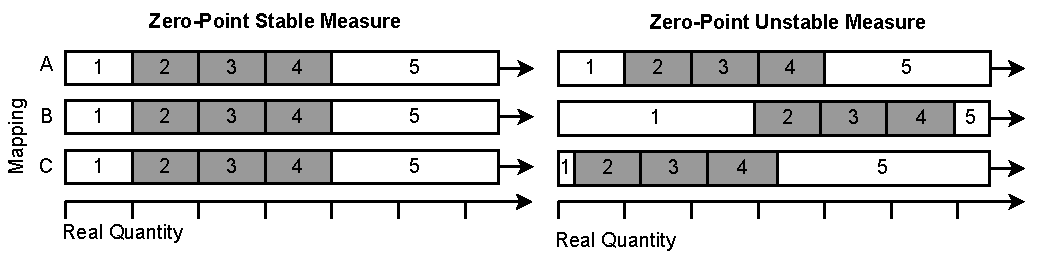
\includegraphics[width=\columnwidth]{Plots/zeropointinstability.pdf}
  \caption{Example of a zero-point stable and a zero-point unstable measure. Note that for each zero-point unstable mapping, all thresholds move up or down by a constant amount ($C_p$ in the equation below).}
  \label{fig:diagram_one}
\end{figure}

\textit{Zero-point instability} means that the zero-point of the mapping is unstable (Figure \ref{fig:diagram_one}). The thresholds move away or towards the absolute zero point of the magnitude of the attribute by a constant amount in a consistent direction. The range of the thresholds will stay identical. Therefore, assuming we have an $n$-level rating scale measurement scale $P$, measure $p$ is equal to:

\[
\begin{cases} 
    1 & q \leq (a + C_{p})\\
    2 & (a + C_{p}) \leq q < (b + C_{p})\\
    3 & (b + C_{p}) \leq q < (c + C_{p})\\
    \cdots & \cdots < \cdots \\
    n & (z + C_{p}) < q\\
\end{cases}.
\]

where set of thresholds $T = \{a, b, c, \cdots, z\}$, $C_{i}$ is the constant for person or moment $p$, $(a + C_{p}) < (b + C_{p}) < (c + C_{p}) < \cdots < (z + C_{p})$, and $q$ is a continuous measure of $Q$. 

\subsubsection{Scaling instability}
\begin{figure}
  \centering
  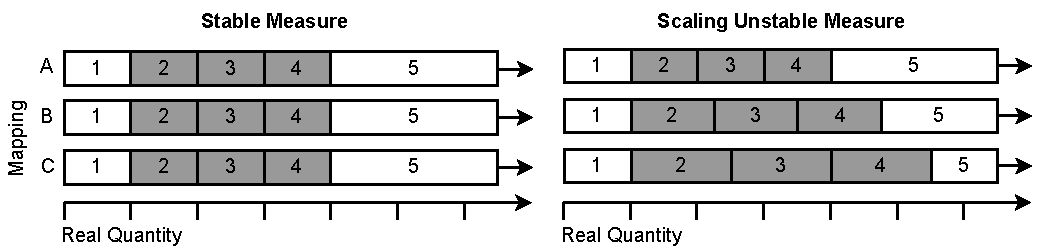
\includegraphics[width=\columnwidth]{Plots/scalinginstability.pdf}
  \caption{Example of a scaling stable and a scaling unstable measure. Note that the threshold range gets scaled up, proportionately distributing the distance between two consecutive thresholds over this range}
  \label{fig:diagram_two}
\end{figure}

\textit{Scaling instability} is instability that comes from a changing distance between the highest threshold and the lowest threshold (the zero-point). The range of the measurement instrument is unstable. In other words, the segment of the quantitative attribute that is mapped to the representation can be wider or more narrow in the quantitative attribute depending on the person or the time point on which a person is measured. Scaling instability is independent of zero-point instability. The difference of each threshold to the lower range bound is scaled up by a common factor. Therefore, assuming we have an $n$-level rating scale measurement scale $P$, measure $p$ is equal to:

\[
\begin{cases} 
    1 & q \leq a\\
    2 & a \leq q < a + x_{p}(b - a)\\
    3 & a + x_{p}(b - a) \leq q < a + x_{p}(c - a)\\
    \cdots & \cdots \ \cdots\\
    n & a + x_{p}(z - a) < q\\
\end{cases}.
\]

where where set of thresholds $T = \{a, b, c, \cdots, z\}$, $x_{i}$ is the scaling factor $x$ for person or moment $p$, $a < a + x_{p}(b - a) < q < a + x_{p}(c - a) < \cdots < x_{p}(z - a)$, and $q$ is a continuous measure of $Q$.

\subsubsection{Interval instability}

\begin{figure}
  \centering
  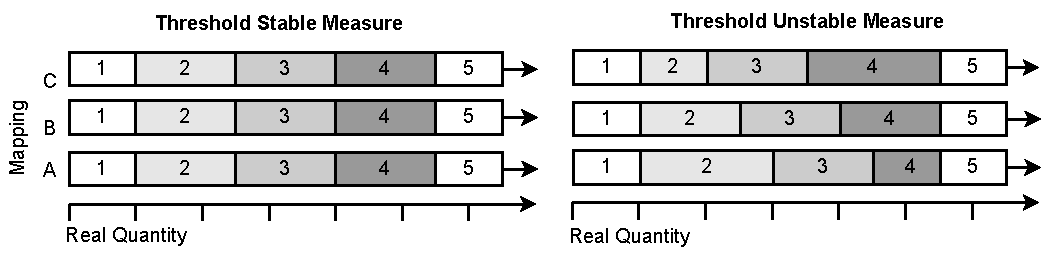
\includegraphics[width=\columnwidth]{Plots/threshold_instability.pdf}
  \caption{Example of a threshold stable and a threshold unstable measure. Note that the range itself does not change, only the distance between consecutive thresholds changes.}
  \label{fig:diagram_three}
\end{figure}

\textit{Interval instability} means that the distance between consecutive pairs of thresholds is not identical. Interval instability can have a structural or a random appearance. An example of structural interval instability would be a growing distance between each subsequent neighbouring pair of thresholds. In random interval instability, there is no relationship between the order of the pairs and the distance of neighbouring pairs of thresholds. The instability is the result of random fluctuations. Interval instability can simultaneously have a structural and a random component. Assuming we have an $n$-level rating scale measurement $P$, measure $p$ is equal to:

\[
\begin{cases} 
    1 & q \leq (a + K_{pa})\\
    2 & (a + K_{pa}) \leq q < (b + K_{pb})\\
    3 & (b + K_{pb}) \leq q < (c + K_{pc})\\
    \cdots & \cdots \leq \cdots\\
    n & (z + K_{pz}) < q\\
\end{cases}.
\]

where the set of thresholds $T = \{a, b, c, \ldots, z\}$, $K_{pt}$ is the constant for person or moment $p$ at threshold $t$, $a + K_{ia} < b + K_{ia} < \cdots < z + K_{iz}$, and $q$ is a continuous measure of $Q$.

\subsubsection{Combinations}
Scores can be higher than the highest thresholds and lower than the smallest thresholds. These scores will naturally be mapped to the lowest or highest option. Second, if the zero-point of the mapping is stable then scaling instability can only affect the right bound of the range. Further, thresholds cannot be outside of the range of the measuring device by definition. Therefore, interval instability is limited by scaling and zero-point instability.

\section{Method}
\subsection{Aims}
The aim of this simulation is to study the statistical consequences of mapping instability on Type-I error and the power. We do two experiments. In the first experiment, we look at what happens when we add random mapping instability for each data point. In the second experiment, we look at what happens when the mapping is unstable between groups. Each experiment has two tests, one where we calculate the Type-I error and one where we calculate the empirical power.

\subsection{Common research set-up for both experiments}
We start by drawing numbers that represent the `magnitudes' for the attributes. We do this by drawing magnitudes from a pre-specified distribution. Then, we map the real value into response categories for 5000 iterations at every combination of a set of degrees of mapping instability. For each iteration, we perform one t-test where there is a difference between the groups to calculate empirical power, and one t-test where there is no difference between the groups. This is used to calculate how the mapping affects the empirical Type I-error rate. Both the empirical power (when there is a difference between the groups) and the Type-I error rate (when there is no difference between the groups) were calculated through the proportion of tests that had a p-value lower than the $\alpha$-rate. Random numbers are generated using the Xoshiro256++ algorithm. The seed is 8508845.
\subsection{Threshold Generation}

\begin{figure}
    \centering
    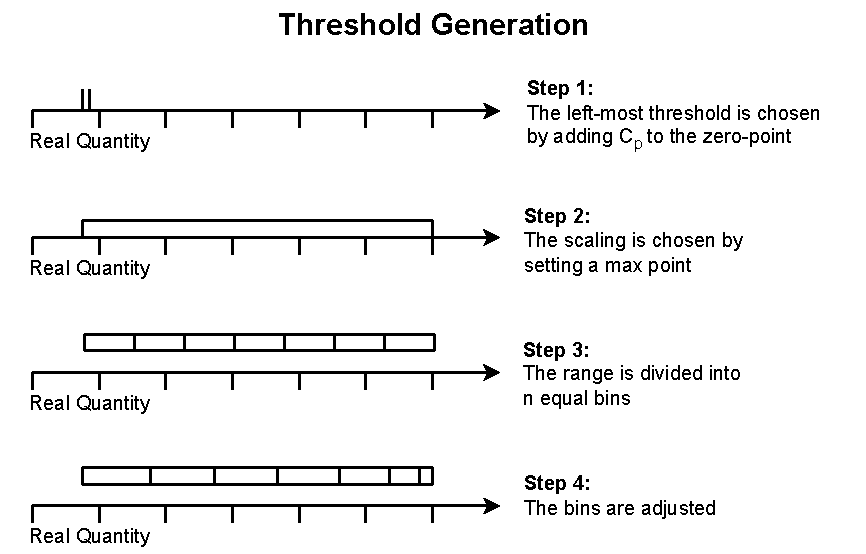
\includegraphics[width=0.5\linewidth]{Plots/threshold_generation.pdf}
    \label{fig:diagram_four}
    \caption{The four stages of the threshold generation process.}
\end{figure}

We emulate differences in the degree of measurement stability by running the thresholds through a transformation pipeline. Each stage of the pipeline draws on the results of the last, until one set of thresholds is left (Figure \ref{fig:diagram_four}). In the first experiment, thresholds are generated for each iteration of the simulation, right before we perform the analysis. In the second experiment, one set of thresholds is generated for each group. We aim to capture a great deal of the distribution, while still keeping discriminative ability. Therefore, we capture 99.7\% of the possible observations in the  standard setting. It captures the distance from 3 $\sigma$ below the mean to three $\sigma$ above the mean with equal intervals. Hence, the zero-point is set to -3, and the scaling is set to 6 (Figure \ref{fig:diagram_five}).

\begin{figure}
    \centering
    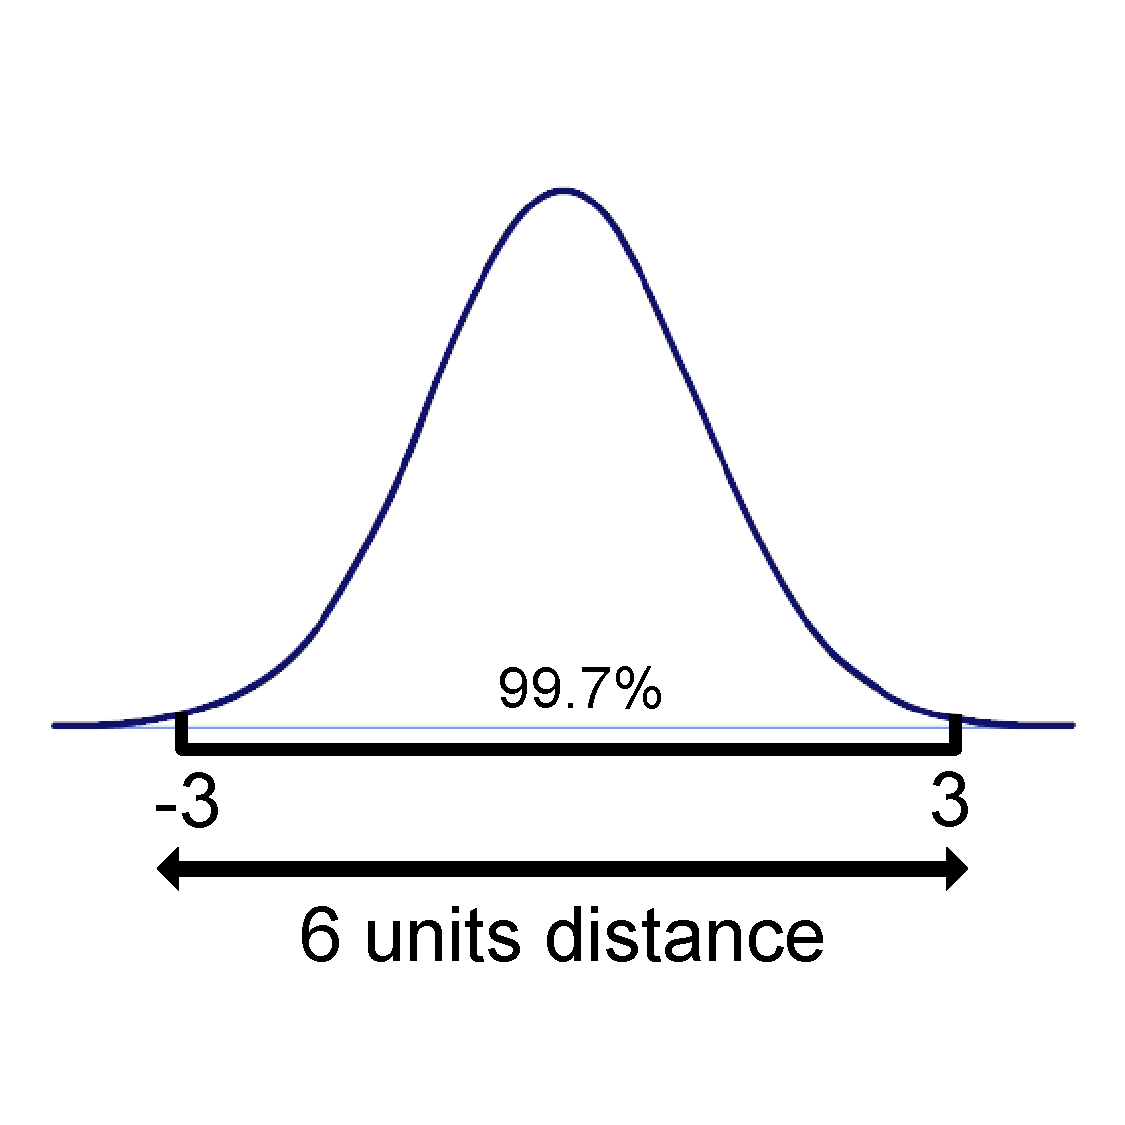
\includegraphics[width=0.25\linewidth]{Plots/justification_for_chosen_distances.pdf}
    \caption{Justification for the default parameters of the simulation. We aim to capture a large part of the distribution, while keeping discriminative ability.}
    \label{fig:diagram_five}
\end{figure}

\subsubsection{\textbf{Step 1:} Setting the zero point}
First, we set the point where the left-most threshold. 

\subsubsection{\textbf{Step 2:} Setting the scaling}
We then set the scaling. This is calculated by adding a constant to the zero-point, effectively setting the range of thresholds: the distance from the smallest to the largest threshold.

\subsubsection{\textbf{Step 3:} Distributing the thresholds}
We set the number of response categories as a parameters for the simulation. This is fed into the function that generates the thresholds.

\subsubsection{\textbf{Step 4:} Adjusting the thresholds}
We generated the thresholds by dividing the distance of the left bound of the range to the right bound of the range by the number of thresholds. Then, the thresholds are transformed through the cumulative distribution function of the beta-distribution. We draw either $\alpha$ and $\beta$ from a normal distribution with a $\mu$ of zero. If we draw a negative number from the distribution, we add its positive equivalent to $\alpha$ and if it is positive we add the number to $\beta$. We chose to use the cdf because it results in either an increasing or decreasing distance between consecutive thresholds over the whole range.

\subsection{Mapping the real scores to the bins}
Afterwards, we map each of the generated values to bins with the generated thresholds as cut-off values. 

\subsection{Experiments}
\subsubsection{Experiment One: Effect of Random Mapping Instability on All Observations}
In experiment one, we added random mapping instability to each observation. For each observation, mapping instability was drawn from the distributions given in Table~\ref{tab:table_one}. 5000 samples were drawn for each combination of parameters $x$, $y$, $z$, and $a$. There was no difference between the mapping instability settings between the two groups. 

\begin{table}
    \centering
    \resizebox{\textwidth}{!}{
    \begin{tabular}{|c||c|c|}
    \hline
    \textit{Concept} & \textit{Variable in equations} & \textit{Parameters}\\
    \hline
    \hline
    \textbf{Zero-point instability} & $C_p$ & \makecell{Normal($-3, x$) \\ where $x \in \{0.2, 0.4, 0.6, 0.8, 1\}$}\\
    \hline
    \textbf{Scaling instability} & $x_p$ & \makecell{Normal($6, y$)  where $y \in \{0.2, 0.4, 0.6, 0.8, 1\}$}\\
    \hline
    \textbf{Number of categories} & Number of elements of $T$ & \makecell{$z$ where $z \in$  $\{4, 5, 6, 7, 8, 9, 10, 11, 12, 13, 14, 15, 20, 50, 80, 100\}$}\\
    \hline
    \textbf{Threshold Instability} & \makecell{$K_{pa}, K_{pb}, K_{pc}, \ldots, K_{pz}$ \\ for categories $a, b, c, \ldots, z$} & \makecell{Normal(0, $a$)  where a$ \in {0.2, 0.4, 0.6, 0.8, 1}$}\\
    \hline
    \end{tabular}}
    \caption{An overview of the settings for the simulation parameters for the first experiment. Each row corresponds to a different concept, with the second column indicating the variable in equations affected by the distribution, and the third column listing the parameters of the distribution. The first column represents the concept that the variable has to represent. The second column is the variable that is being set using the distribution. Note that threshold instability has a pretty specific implementation (see step 4 of the threshold generation section).}
    \label{tab:table_one}
\end{table}

\subsubsection{Experiment Two: Effect of Between-Group Mapping Instability}
For experiment two, we added structural differences in the mapping between the two experimental conditions. The mapping was kept stable within each group. The parameters of the two groups are given in Table~\ref{tab:table_two}. There was no fluctuation within the groups. 5000 samples were drawn for each combination of parameters $x$, $y$, $z$, and $a$. 

\begin{table}
    \centering
    \resizebox{\textwidth}{!}{
    \begin{tabular}{|c||c|c|c|}
    \hline
    \textit{Concept} & \textit{Variable in equations} & \textit{Group 1} & \textit{Group 2} \\
    \hline
    \hline
    \textbf{Zero-point instability} & $C_p$ & $-3$ (3 $\sigma$ below $\mu$)& \makecell{$x$ where $
    x \in \{-3.5, -3.4, -3.3, -3.2, -3.1, -3.0,$ \\ $-2.9, -2.8, -2.7, -2.6, -2.5\}$}\\
    \hline
    \textbf{Scaling instability} & $x_p$ & 6 (3 $\sigma$ above $\mu$)& \makecell{
    $y$ where $y \in \{5.5, 5.6, 5.7, 5.8, 5.9, 6.0,$\\
    $6.1, 6.2, 6.3, 6.4, 6.5\}$} \\
    \hline
    \textbf{Number of categories} & Number of elements of $T$ &
    \makecell{
    $z$ where $z \in$ \\
    $\{4, 5, 6, 7, 8, 9, 10, 11, 12,$ \\ $13, 14, 15, 20, 50, 80, 100\}$}
    & \makecell{
    $z$ where $z \in$ \\
    $\{4, 5, 6, 7, 8, 9, 10, 11, 12,$ \\ $13, 14, 15, 20, 50, 80, 100\}$} \\
    \hline
    \textbf{Threshold Instability} & \makecell{
    $K_{pa}, K_{pb}, K_{pc}, \ldots, K_{pz}$ \\
    for categories $a, b, c, \ldots, z$} & 0.0 (equal thresholds)& \makecell{$a$ where  $a \in$ \\ $\{-0.5, -0.4, -0.3, -0.2, -0.1,$\\$ 0.0, 0.1, 0.2, 0.3, 0.4, 0.5\}$} \\
    \hline
    \end{tabular}}
    \caption{An overview of the simulation parameters for the second experiment}
    \label{tab:table_two}
\end{table}

\subsection{Analysis}

\begin{figure}
    \centering
    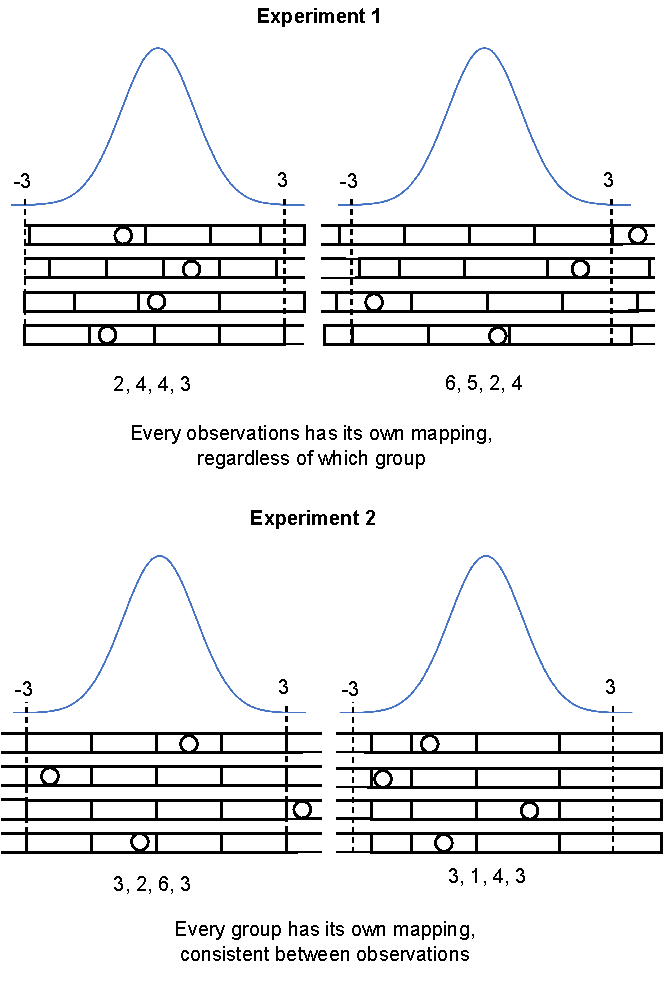
\includegraphics[width=0.5\linewidth]{Plots/difference_between_experiments.pdf}
    \caption{An illustration of the difference between the experiments.}
    \label{fig:diagram_six}
\end{figure}

Each iteration, we perform the same two tests given a certain combination of parameters. We simulate a simple independent-sample t-test so that each test is close to a statistical power of 0.80 for a one standard deviation difference between samples based on an $\alpha$ of 0.05. Our sample size is 18 participants per group. These two tests are performed in both experiments.

In the first test, two samples of magnitudes are drawn from the same normal distribution. The test has an $\alpha$ of 0.05. We draw both samples from a standardised normal distribution:

    \centerline{Normal ($\mu$ = 0; $\sigma$ = 1)}

In the second test, there is a one standard deviation difference between the null distribution and the alternative distribution. Given our sample size, our test should find a difference in 80.7\% of the cases. The parameters are as follows:

    \centerline{Group 1:\@ Normal ($\mu = 0; \sigma = 1$)}
    \centerline{Group 2:\@ Normal ($\mu = 1; \sigma = 1$)}

\subsection{Software}
We used the Julia language, and in particular the `Statistics.jl' and `HypothesisTests.jl' packages, to set up the simulation and to run the statistical analysis~\citep{bezanson_julia_2017}. Analyses were run on a personal computer through a Pluto-notebook. Instructions for running the analysis through a sandboxed project environment identical to our system can be found on the main page of \href{https://github.com/MvanSteenbergen/MappingInstability}{a Github repository}. Both the distributions and the test were chosen to use simple, commonly known statistics with the aim to show the potential consequences of zero-point, scaling, and interval instability. The experiment can be repeated using any possible test: the values are mapped \textit{before} the analysis is run, so the full study is independent of the hypothesis testing procedure. The study was approved by the Ethical Review Board of the Faculty of Social and Behavioural Sciences of Utrecht University (23-1844).

\section{Results}
\subsection{Experiment 1: Adding Random Mapping Instability To All Observations}

\begin{figure}
    \centering
    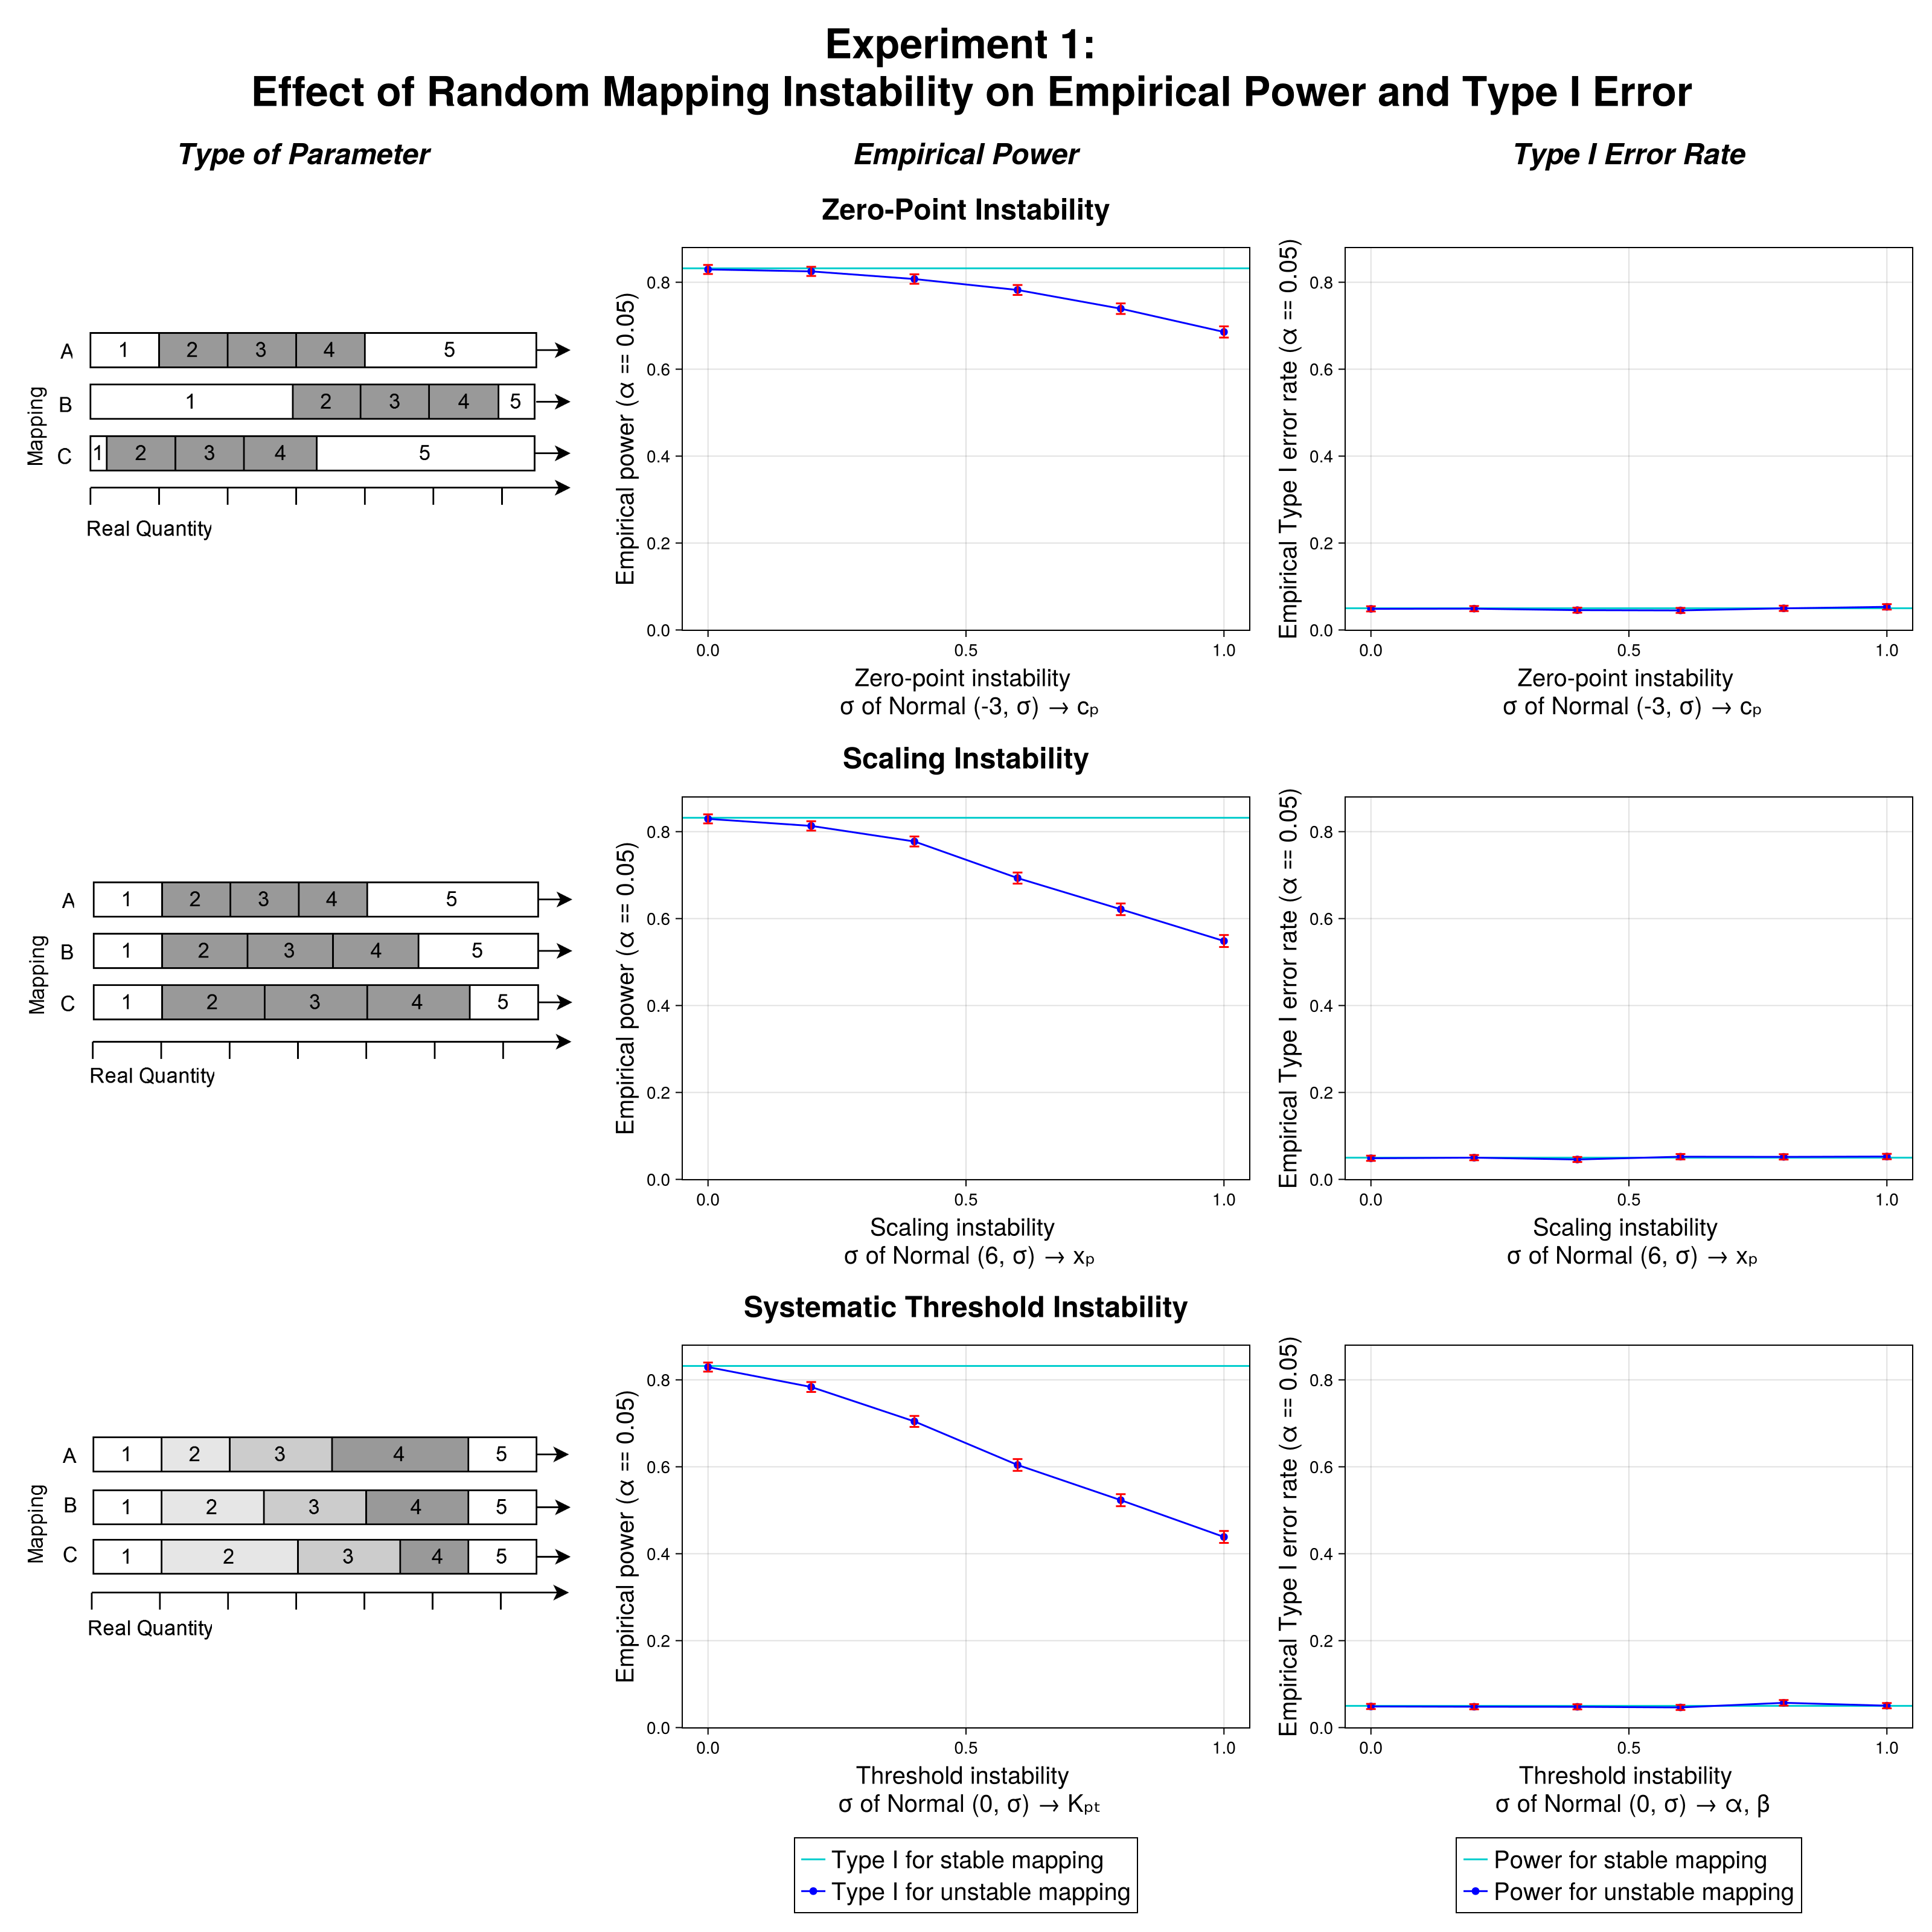
\includegraphics[width=1\linewidth]{Plots/measurement_instability_random.png}
    \caption{This figure illustrates the influence of three sub-types of mapping instability on statistical power and Type I error rate. The x-axis of each plot indicates the severity of mapping instability that is drawn from a distribution for each observation independent of group-membership. The y-axis represents either the Type I error rate or statistical power. The light-blue lines represent the value for the test if no mapping takes place. The red error-bars represent the 95\% confidence interval. Power goes down when mapping instability is added. The Type I error rate does not significantly change.}
    \label{fig:plot_one}
\end{figure}

We first tested how the different types of mapping instability affect Type I error (when both groups are drawn from identical distributions) and power (when the groups are drawn from two different distributions). Our results suggest that the Type I-error rate is not significantly affected by zero-point instability (Figure \ref{fig:plot_one}). It is flat over the whole range for each mapping instability parameter. As expected, power generally becomes lower when mapping instability is higher, monotonically decreasing when instability increases.  Two-way interactions between power and the different sub-types of mapping instability indicate that the effect on power becomes stronger if different levels of threshold instability are combined ~(Figure~\ref{fig:plot_two}). There is no noticeable interaction between the number of categories and the mapping instability parameters. These findings suggest random mapping instability only affects power, meaning that if only random mapping instability were present more observations would be needed to find results. 

\begin{figure}
    \centering
    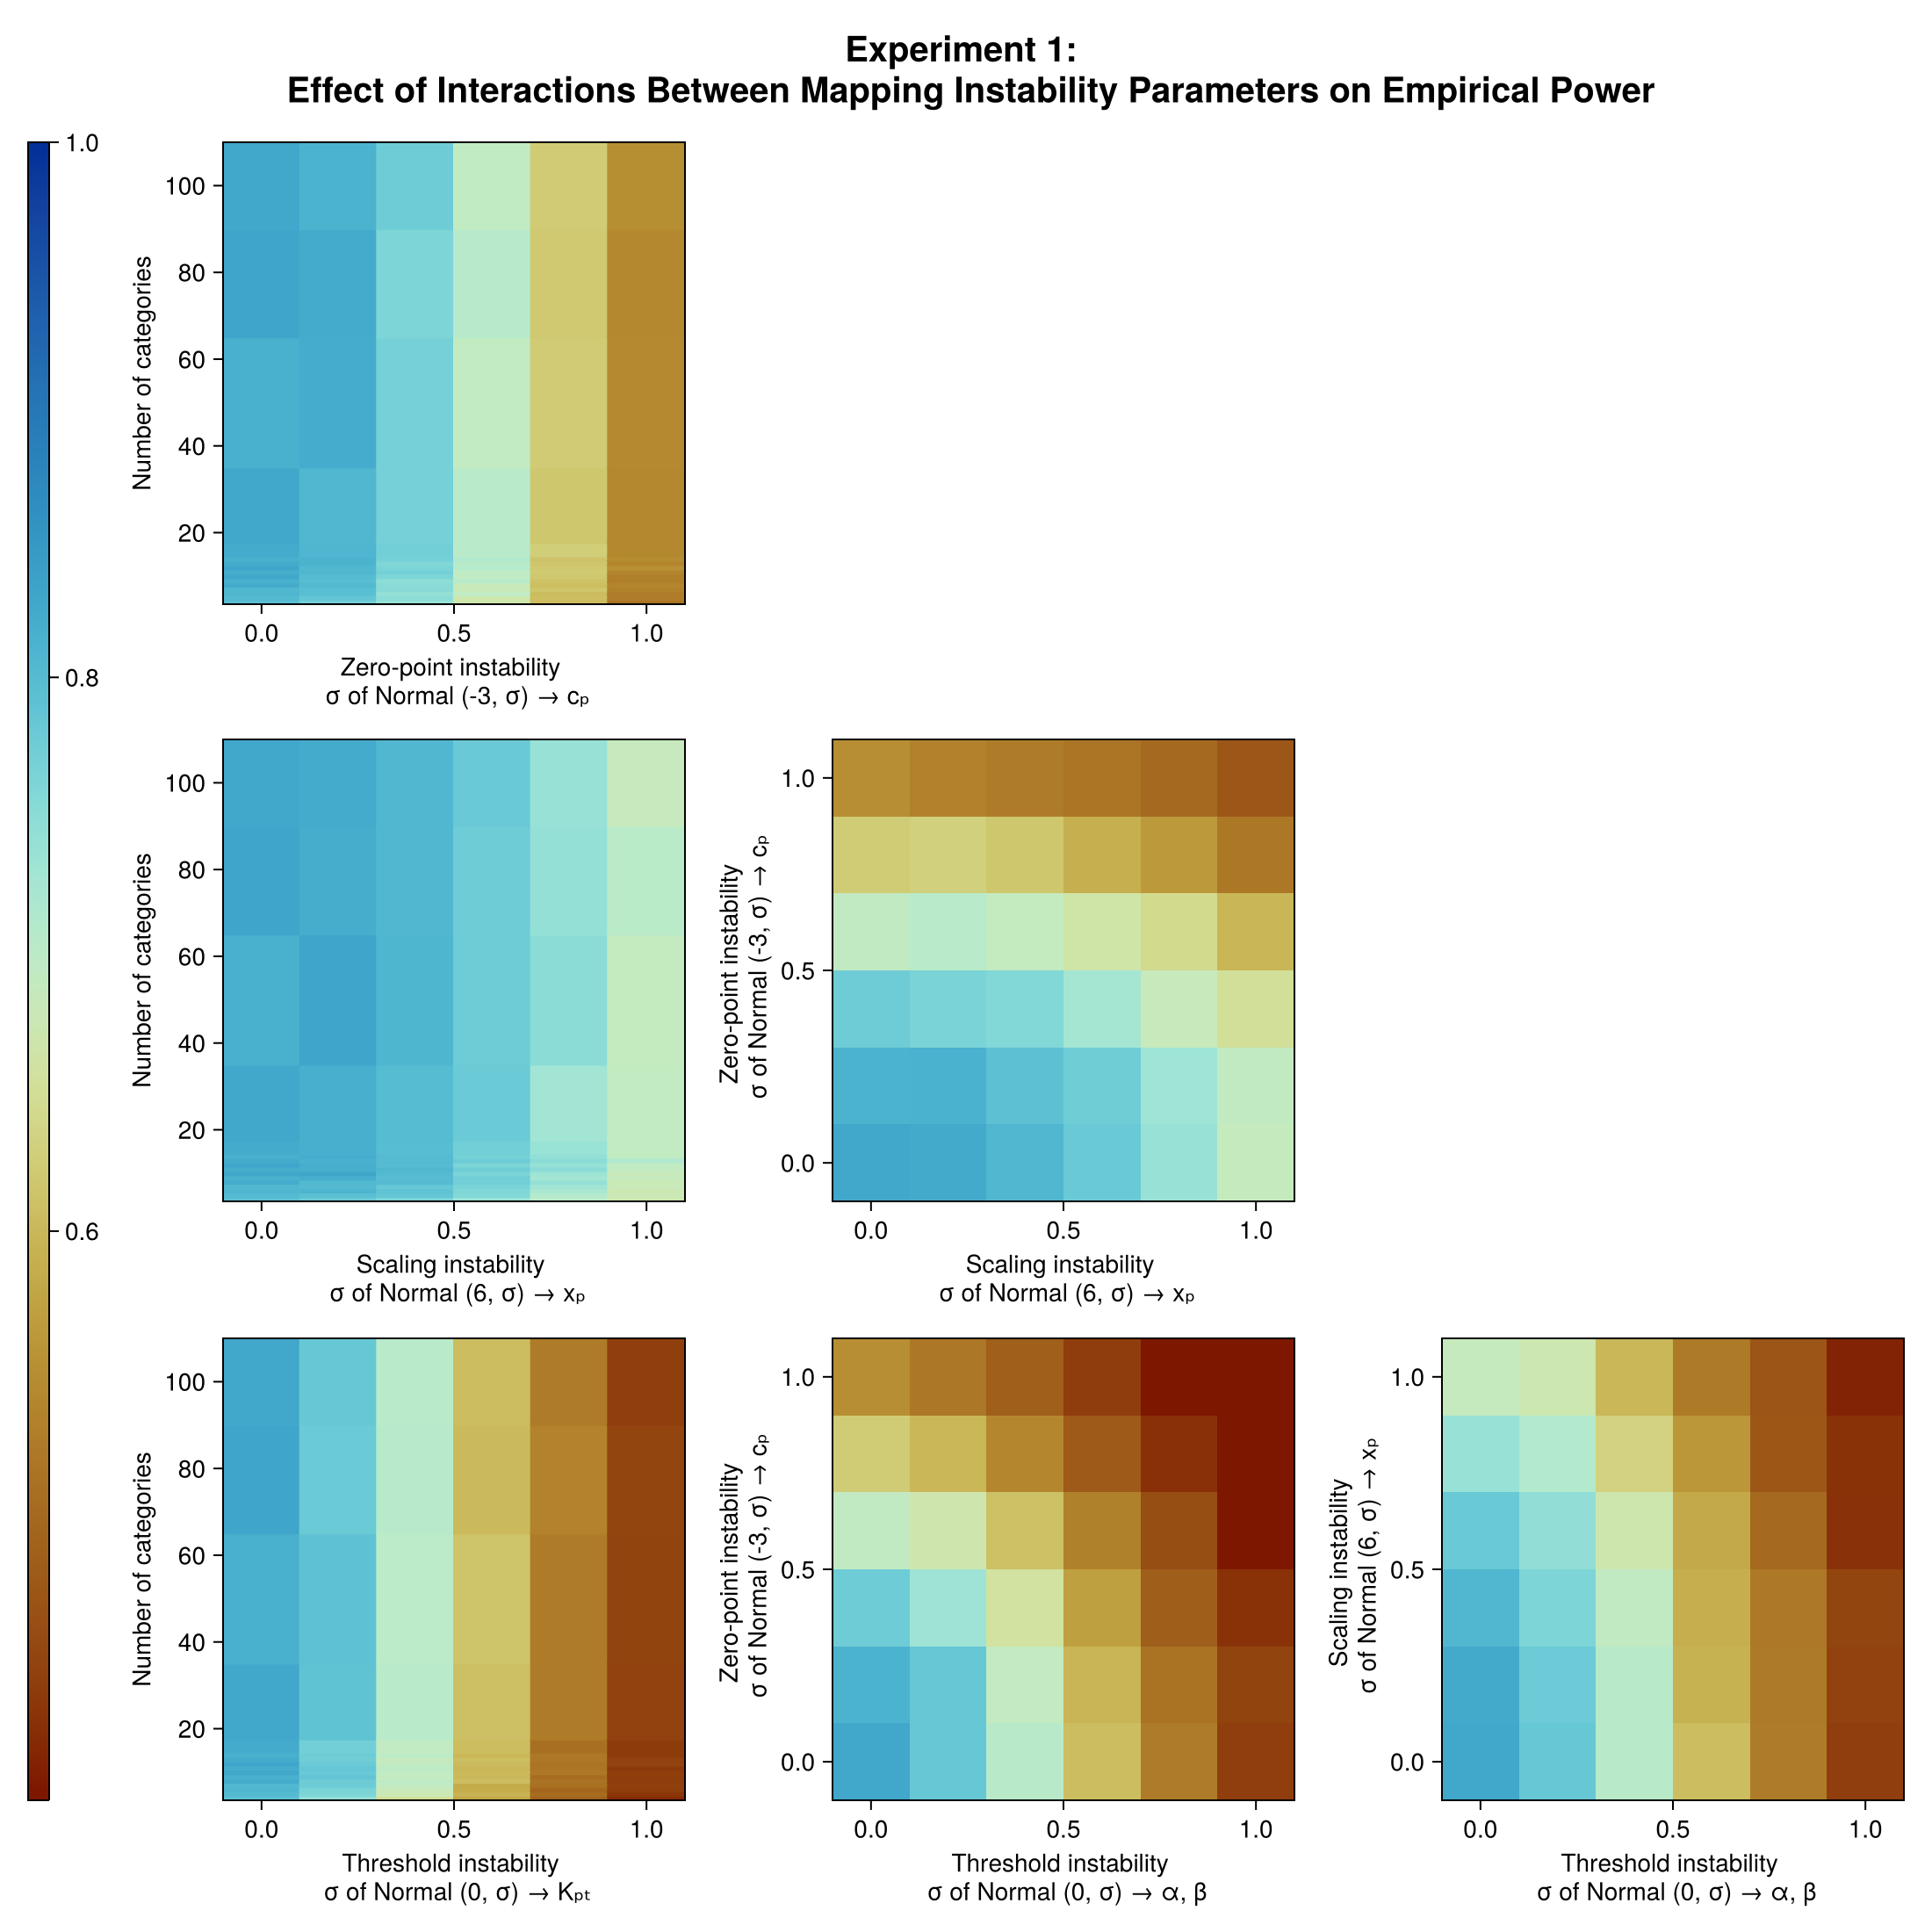
\includegraphics[width=1\linewidth]{Plots/Interactions_measurement_instability_power.png}
    \caption{Heatmaps that showcase the interaction between simulation parameters zero-point instability, scaling instability, threshold instability, and the number of thresholds on the effects of random mapping instability on power. The x-axes and y-axes of each plot represent two simulation parameters, representing the level of mapping instability. The cell colour represents the strength of the power.}.
    \label{fig:plot_two}
\end{figure}

\begin{figure}
    \centering
    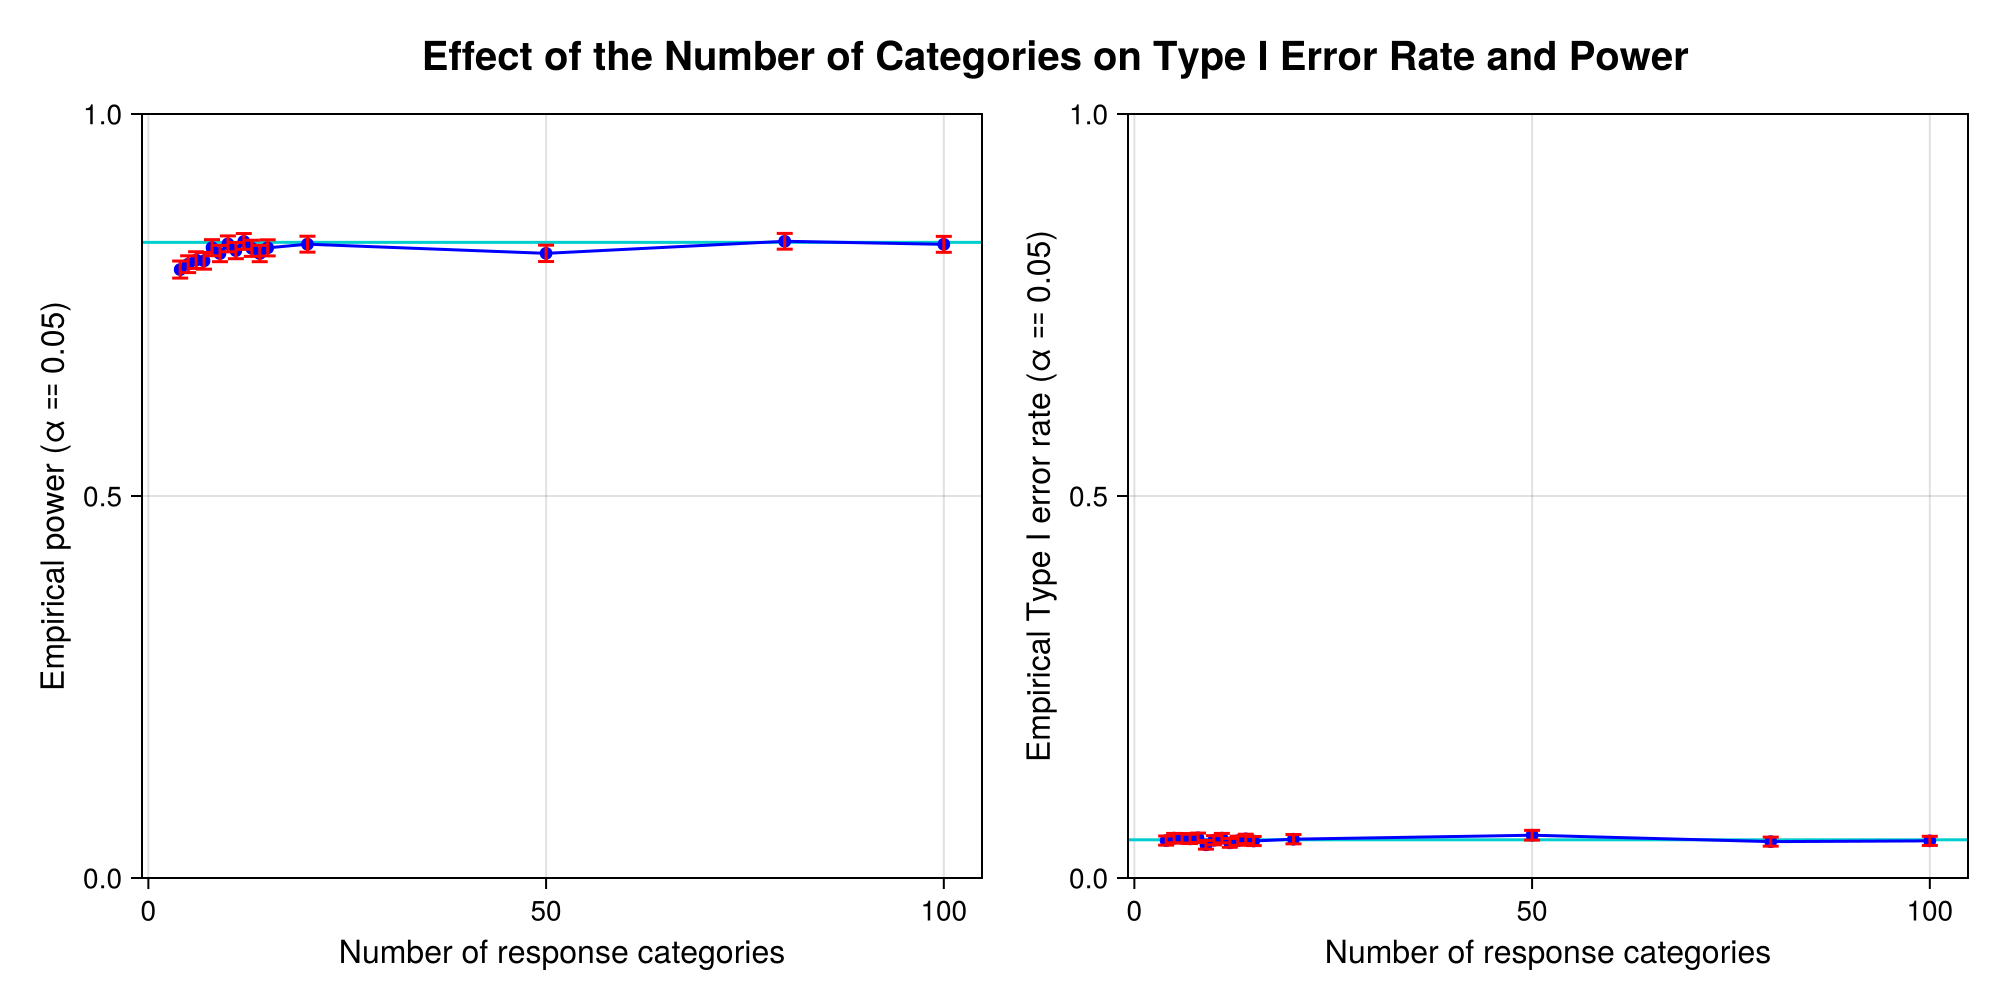
\includegraphics[width=0.75\linewidth]{Plots/nCategories_and_power_typeI.png}
    \caption{In this plot, no mapping instability takes place. }
    \label{fig:plot_three}
\end{figure}

Figure~\ref{fig:plot_three} displays the relationship between the number of categories and the power, and the number of categories and the Type I error rate. It indicates that power is not greatly affected by discretization, not going below 5\% less than the original power. Even when the number of categories is 4, the Type-I error rate is not affected by discretization. For equally spaced intervals, the number of categories by itself has very little bearing on the Type I-error rate and a small influence on the power. It does not affect power when the number of bins becomes higher than 11

\subsection{Experiment 2: Adding Mapping Inconsistency Between the Two Groups}
In the second experiment, we add mapping instability to the two experimental conditions separately. Our results suggest that both power and Type-I error rate are affected by group-based mapping instability (Figure~\ref{fig:plot_four}. Power monotonically decreases from 1 to 0, intersecting with the analysis performed on unmapped variables when no mapping instability is present. The Type-I error rate concaves upward, with 0.05 at the center, indicating that Type-I error grows when the distance is larger from the center point, regardless of sign. Scaling instability influences the type I error rate and power more strongly. For systematic threshold instability, small deviations have a large impact on the Type-I error rate, regardless of whether the thresholds are compressed to the left or compressed to the right. These results suggest that it is crucial to minimise mapping instability between groups, because mapping instability makes the probability of observing Type-I error higher than the $\alpha$ of $0.05$, decreasing the validity of the testing procedure. The interaction plot indicates that interactions between threshold instability, scaling instability, and zero-point instability are quite strong (Figure \ref{fig:plot_five} \& \ref{fig:plot_six}). The different types of mapping instability can strengthen each other, but also weaken each other by cancelling each other out. 

\begin{figure}
    \centering
    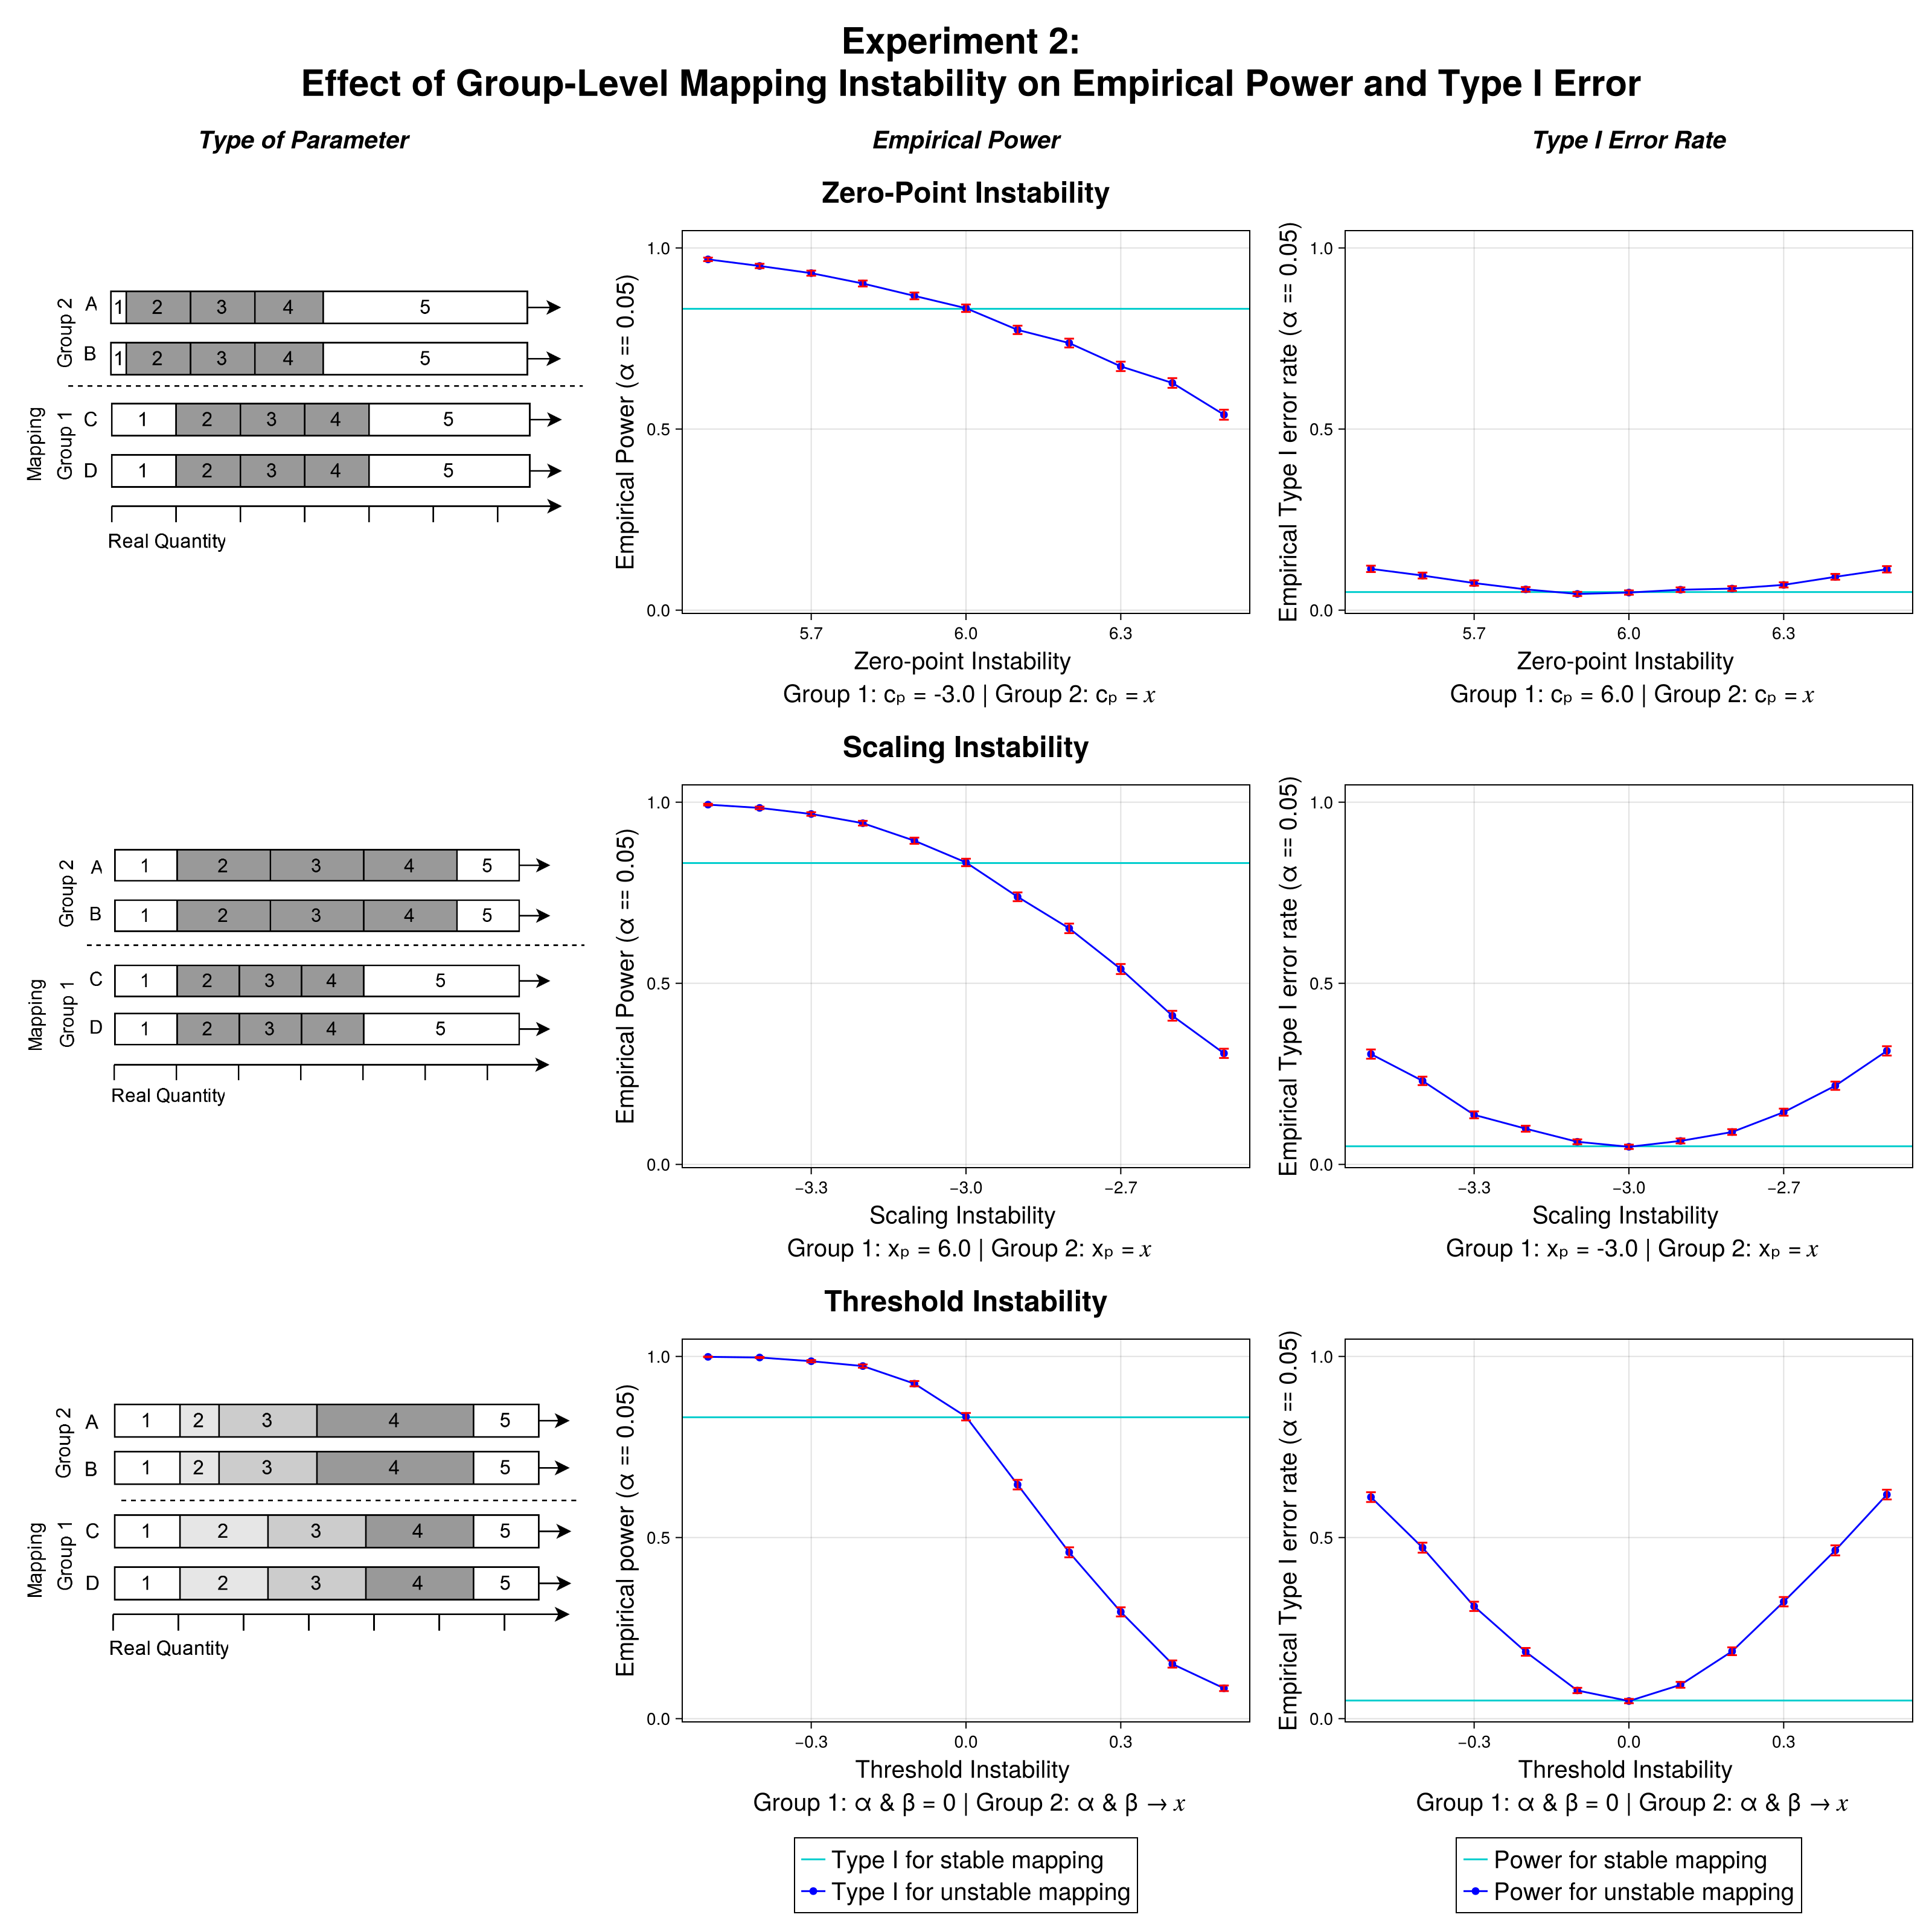
\includegraphics[width=0.9\linewidth]{Plots/measurement_instability_group_based.png}
    \caption{This figure illustrates the influence of three sub-types of mapping instability on statistical power and Type I error rate. Mapping instability concerns inconsistencies in mapping from the `magnitude' to the rating scale categories. These are presented if Table \ref{tab:table_two}. The x-axis of each plot indicates the severity of mapping instability that is applied to the groups. The y-axis represents either the Type I error rate or statistical power. The light-blue lines represent the value for the test if no mapping takes place. The red error-bars represent the 95\% confidence interval. Power goes down when mapping instability makes the condition to which it is applied closer to distribution to which it is not applied. The Type-I error rate goes up when more mapping instability is added.}
    \label{fig:plot_four}
\end{figure}


\begin{figure}
    \centering
    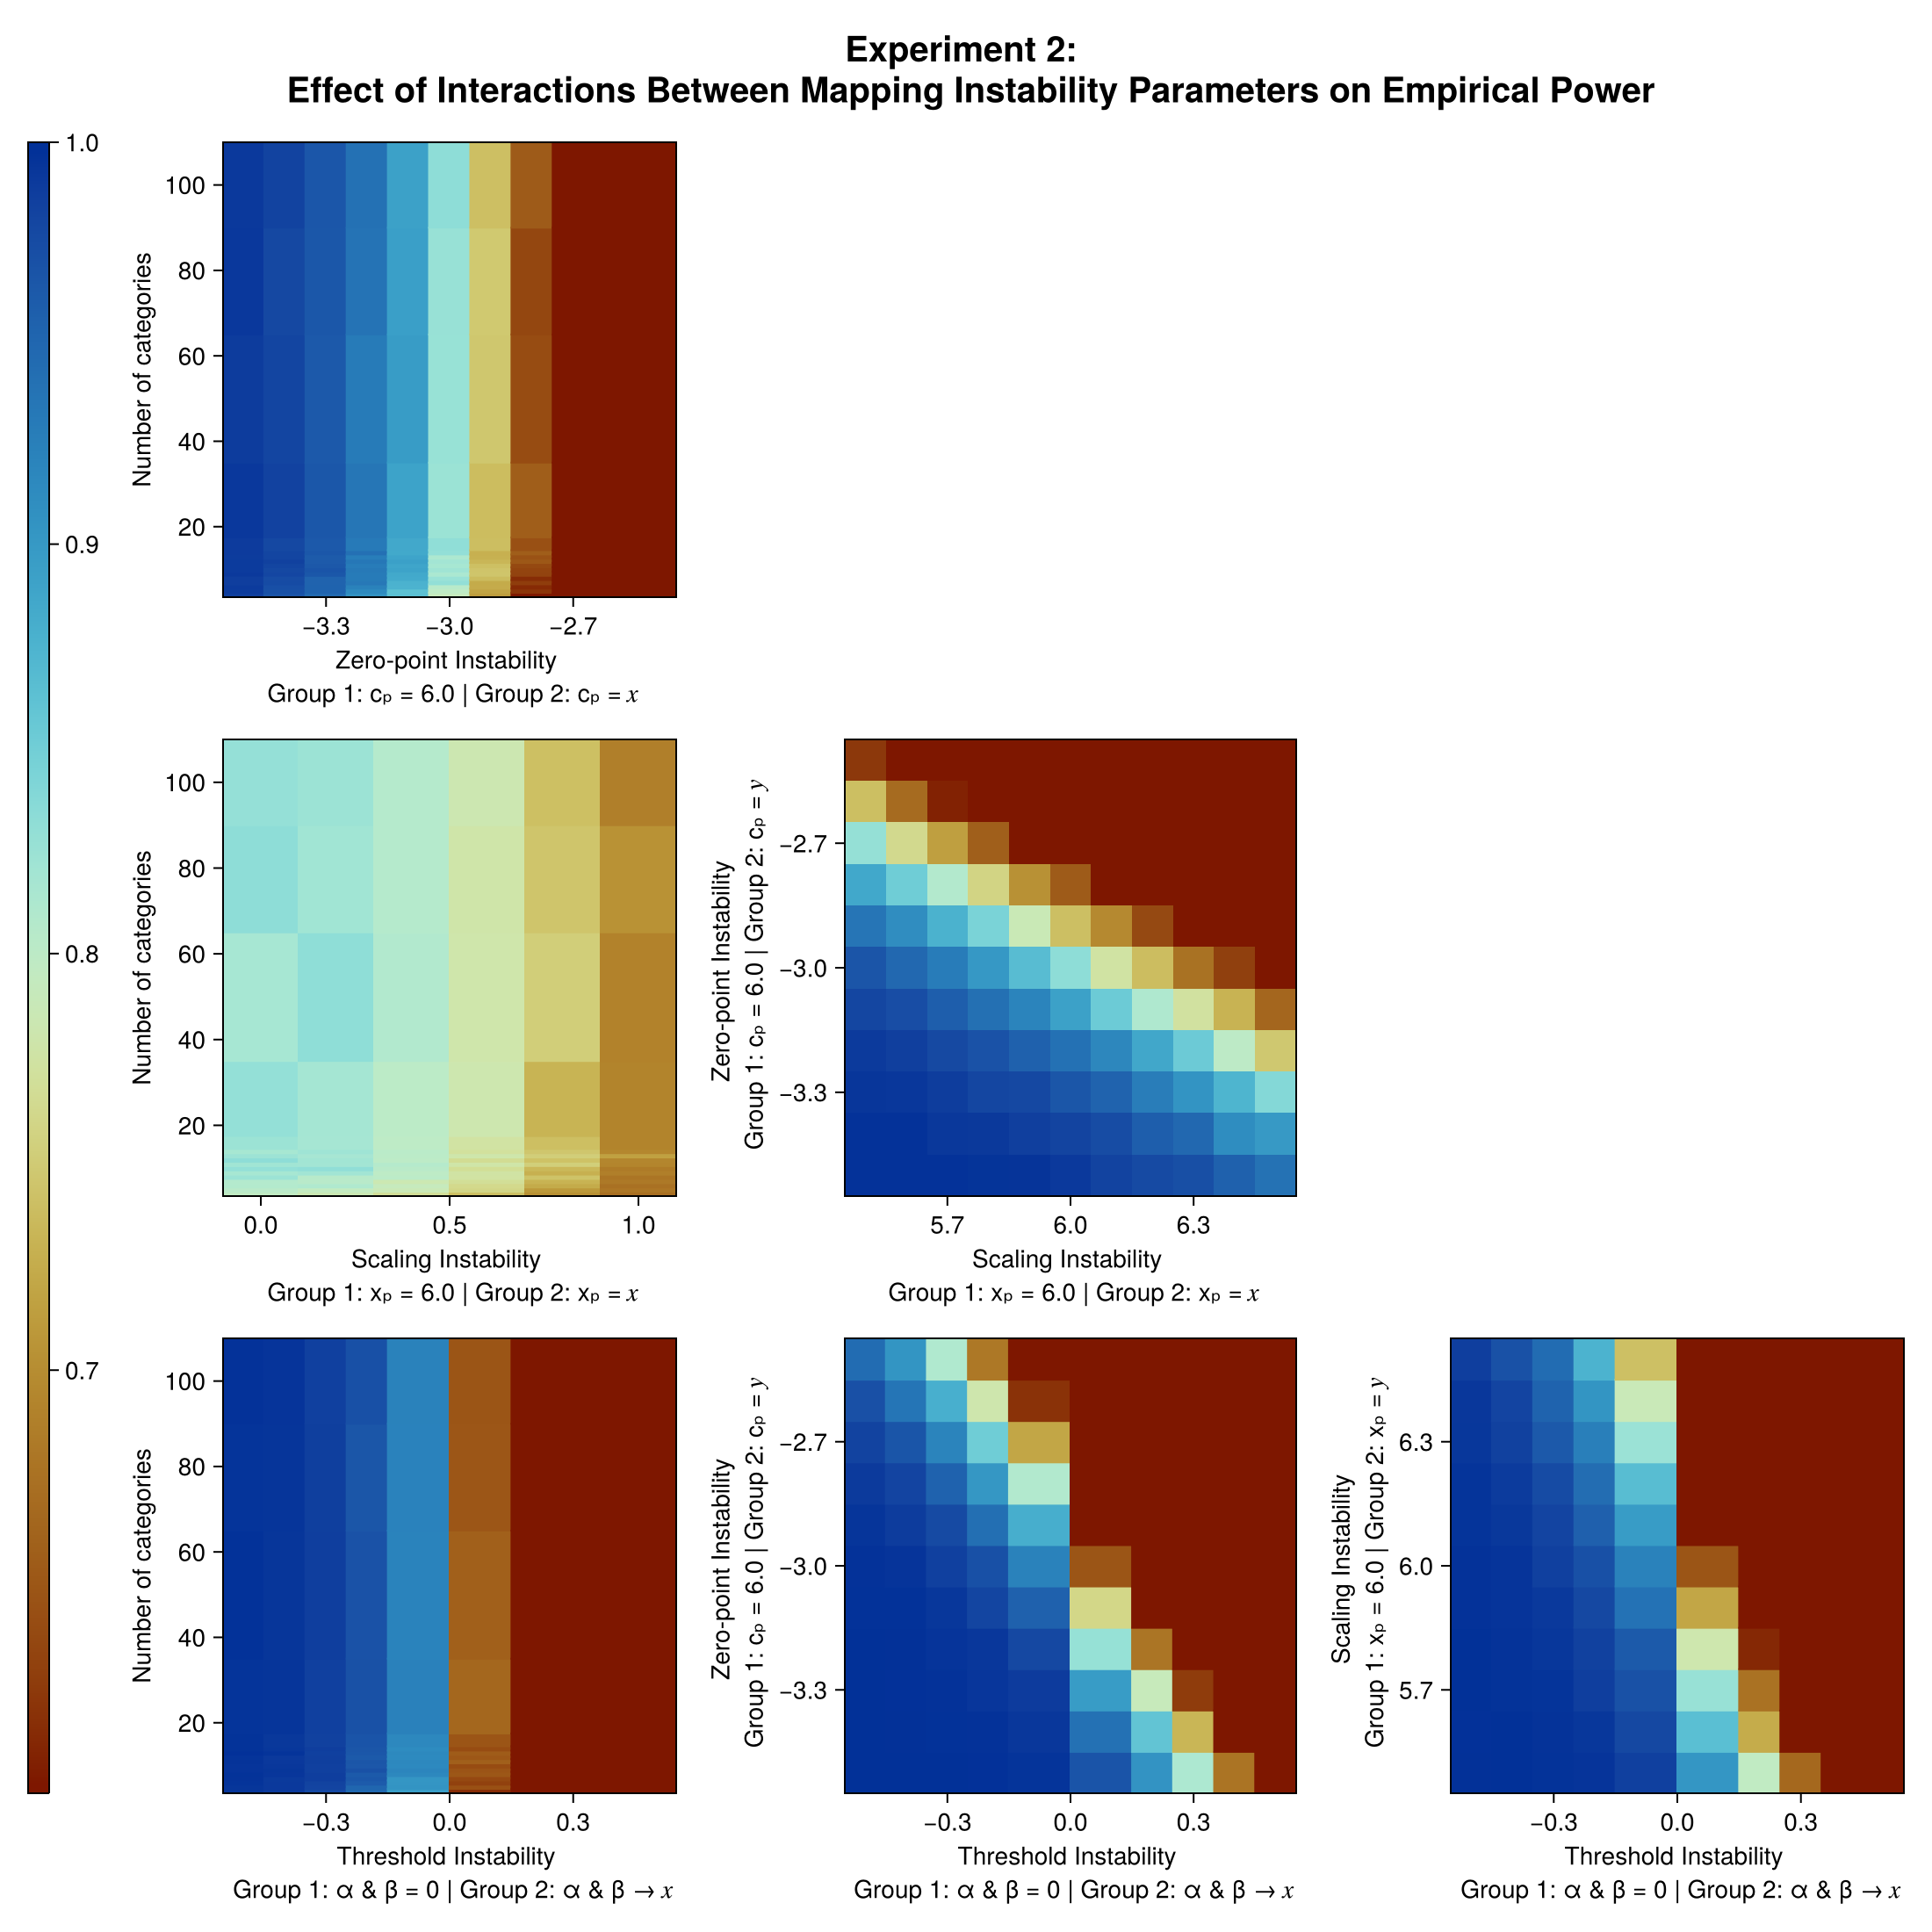
\includegraphics[width=1\linewidth]{Plots/Interactions_measurement_instability_power_group_based.png}
    \caption{Heatmaps that showcase the interaction between simulation parameters zero-point instability, scaling instability, threshold instability, and the number of thresholds on the effects of group-based mapping instability on power. The x-axes and y-axes of each plot represent two simulation parameters, representing the level of mapping instability. The cell colour represents the strength of the power.}
    \label{fig:plot_five}
\end{figure}


\begin{figure}
    \centering
    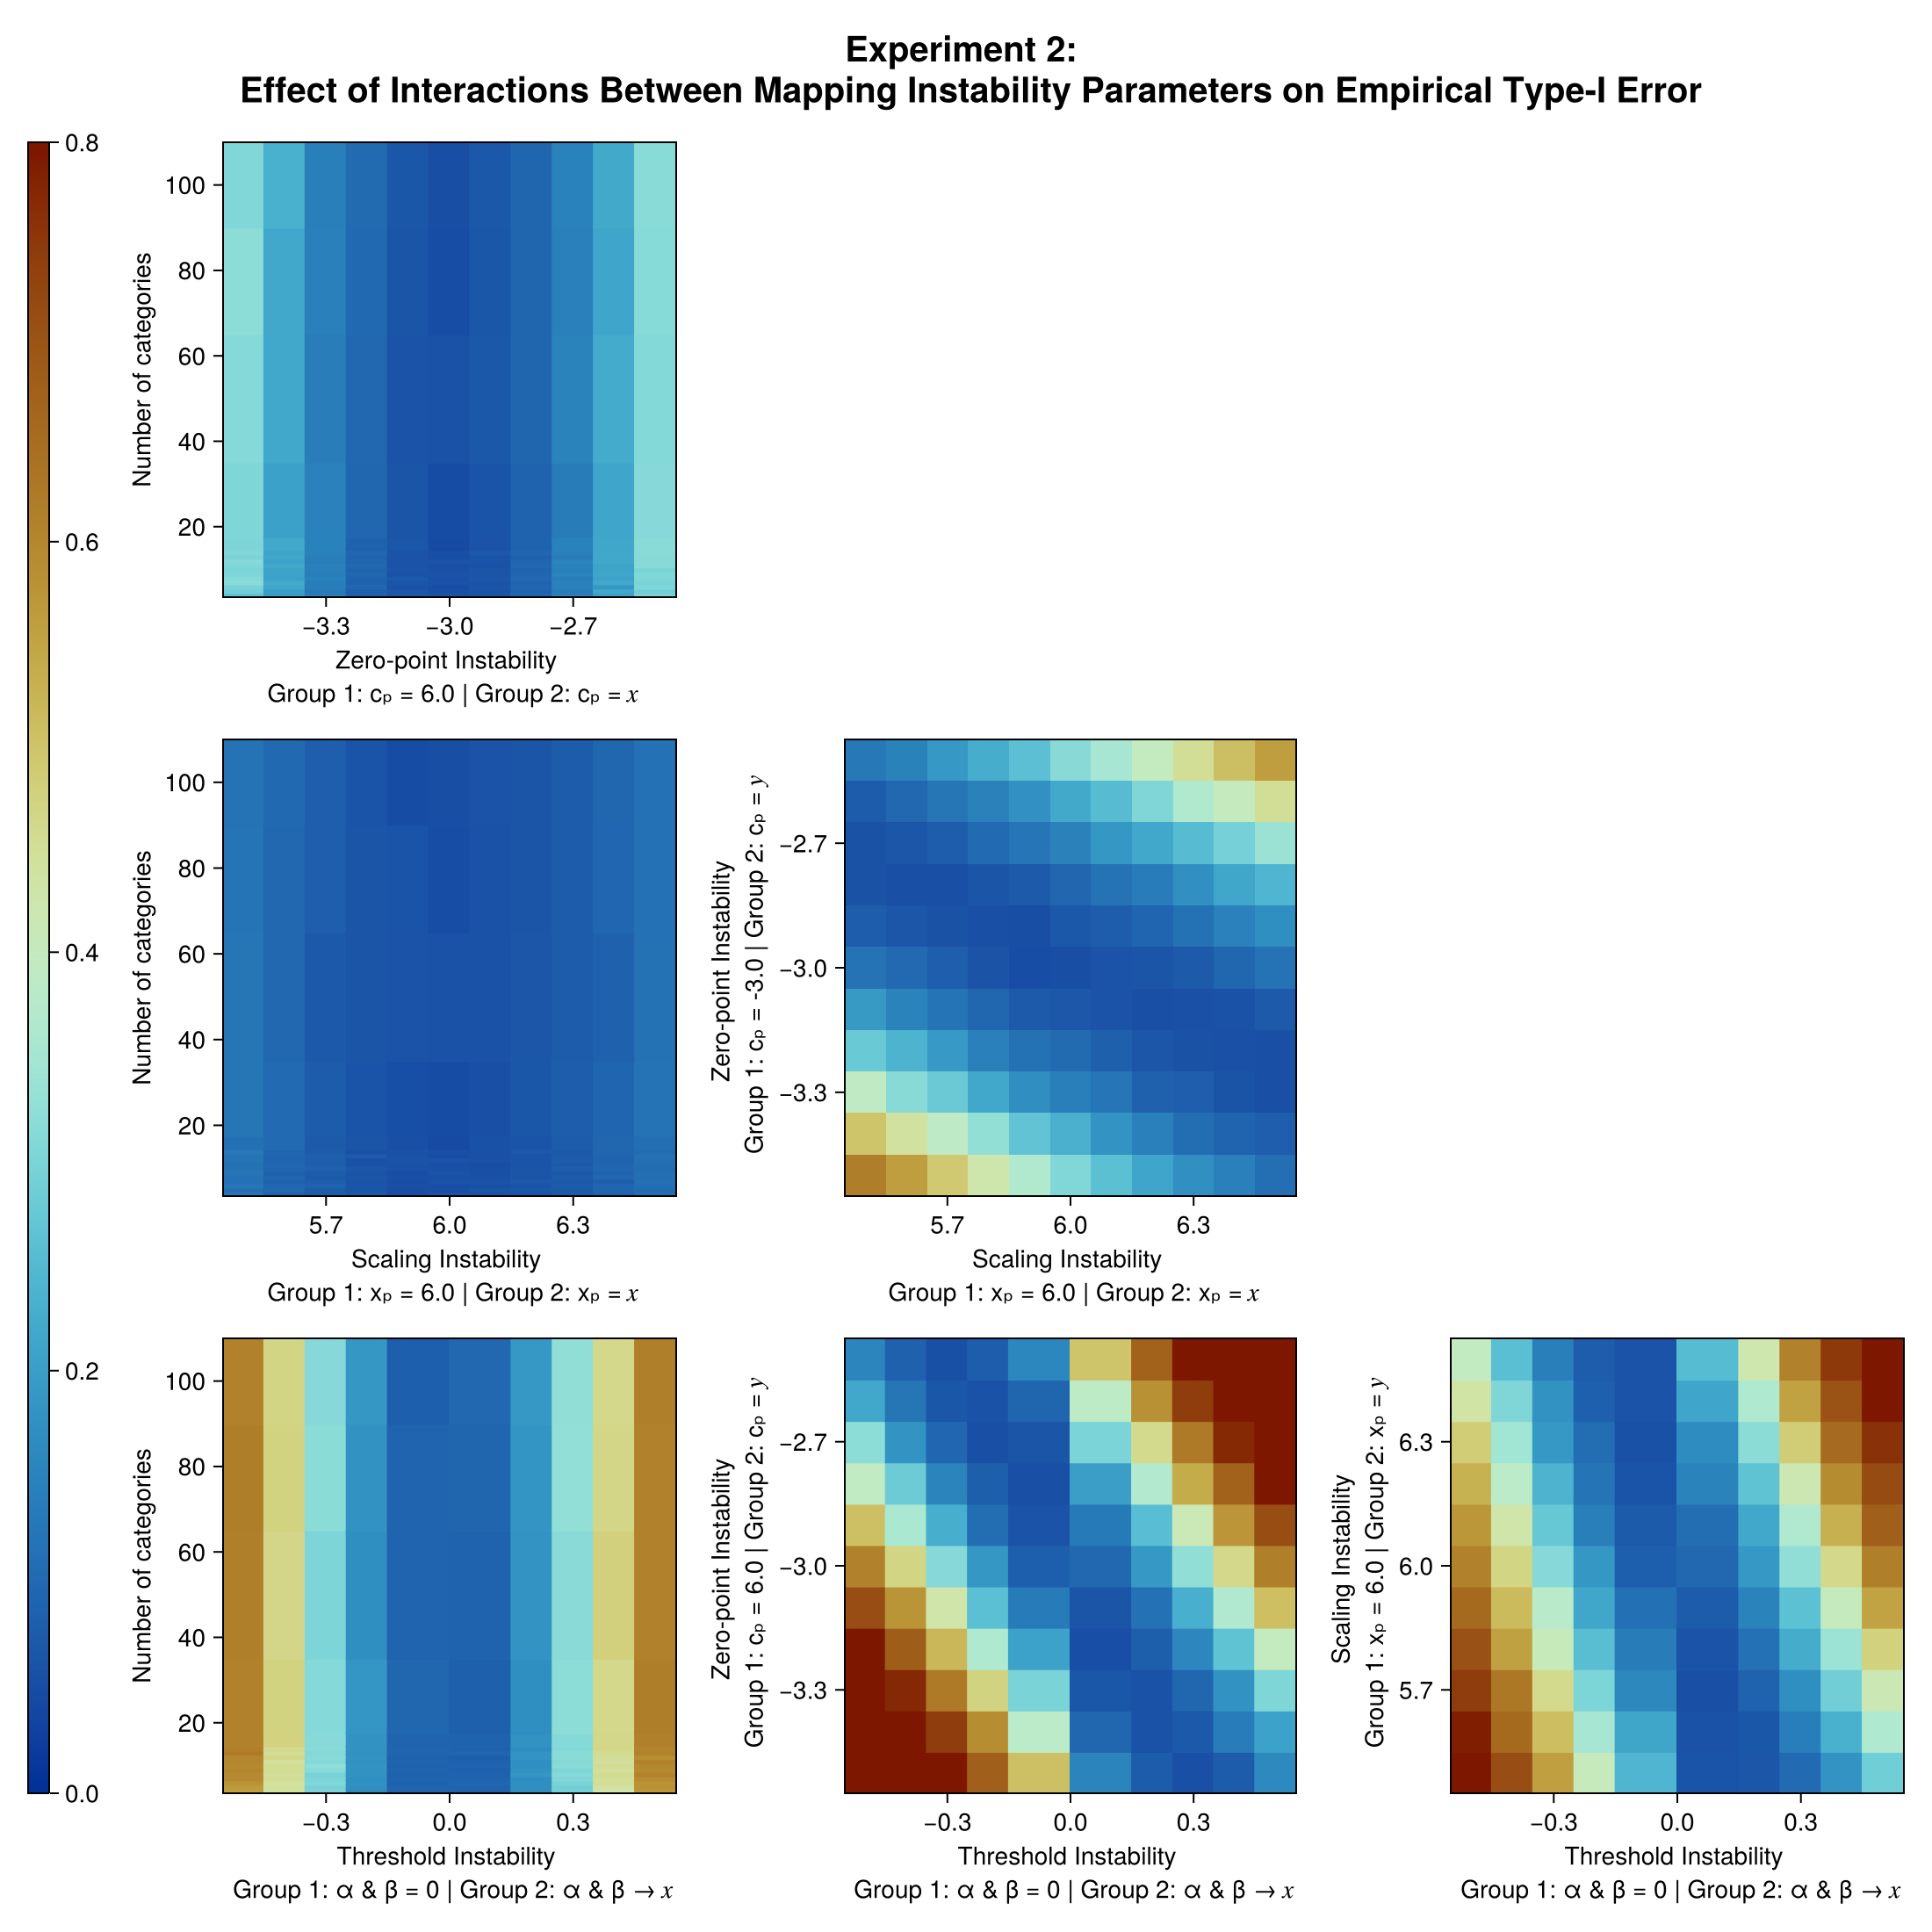
\includegraphics[width=1\linewidth]{Plots/Interactions_measurement_instability_typeI_group_based.png}
    \caption{Heatmaps that showcase the interaction between simulation parameters zero-point instability, scaling instability, threshold instability, and the number of thresholds on the effects of group-based mapping instability on Type-I error. The x-axes and y-axes of each plot represent two simulation parameters, representing the level of mapping instability. The cell colour represents the strength of the Type-I error rate.}
    \label{fig:plot_six}
\end{figure}

\section{Discussion}
We studied the consequences of mapping instability from the magnitude of an attribute to rating scales. The chance of Type-I errors is not impacted by randomly distributed mapping instability. However, because mapping instability increases the amount of variance, a larger number of observations is needed to find effects of the same size. If mapping instability is related to the experimental conditions, mapping instability affects the error rate and the power. These findings emphasise the importance of establishing a clear relationship of the rating scale items to the magnitude of quantitative attributes, by showing that inconsistencies in mapping can lead to incorrect conclusions. 

Modern simulation studies examining the effects of ordinality on measurement implicitly assume a consistent mapping from magnitude to ordinal measure~\citep{kindermann_reliability_2023, wu_can_2017}. Our results suggest that this assumption is not necessarily met, and care is needed to interpret their findings. Standard recommendations should be treated with caution. The Mann Whitney U-tests or other non-parametric equivalents to statistical tests, which are often recommended for rating scale analysis when the outcome does not appear normal, assume rank order \citep{mann_test_1947}. As we have shown, rank order can be compromised if the data results from datasets with inconsistent mappings. This can affect statistical results. Hence, non-parametric methods are not necessarily robust against mapping instability. On a positive note, we see that Type-I error does not go up if mapping instability is unrelated to statistical parameters. 

\subsection{Theoretical Implications}
Our results can be used to bridge two different schools in psychological thought, because it combines elements of both Representational Theory of Measurement and psychometrics. Adherents of the representational theory of measurement study the relationship between the measured attribute and the measurement device. Psychometricians focus on the development and validation of tests to measure psychological constructs. The mapping instability framework uses insights from both to study a real problem in psychology: measurement error and bias. We start from the formal relationship between the magnitude of an `attribute` to the measurement device, building up to a psychometric focus on the relationship of test scores to the underlying psychological constructs in the context of testing. 

The Representational Theory of Measurement has been challenged as a comprehensive measurement framework for psychology, because of its inability to represent error properly~\citep{helzner_representation_2012}. Critics also argue that measurement procedures are not developed by formal reasoning about the structure of empirical relationships~\citep{borsboom_why_2004}. Psychometrics, conversely, has been challenged from the perspective that it makes no direct reference to the empirical structure that underlies measurement and does not have units~\citep{humphry_role_2011}. This makes it difficult to interpret what error means within a psychometric context, because it is unclear on what scale or unit the error is and what the `true score' of an attribute represents. Our approach can lead to clarity in ongoing discussions~\citep{vessonen_psychometrics_2017}. From RTM, we learn what it means to capture a qualitative attribute in a numerical representation. The unit of our quantitative attribute has a clear place in the simulation. We follow Vessonen by arguing that RTM and the psychometric literature can be complementary. RTM can provide the formal conditions for measurement, while psychometrics can provide the evidence for or against those formal conditions~\citep{vessonen_complementarity_2020}. From RTM, we adopt the means to capture a qualitative attribute in a numerical representation. From psychometrics, we adopt the focus on inconsistencies in how participants relate to measurement. We use this to show how formal approaches to measurement can be used fruitfully in psychometric practice.

\subsection{Practical Implications}
The mapping instability framework can serve as a theoretical and pedagogical tool to reframe discussions about error for rating scale devices. Traditionally, the emphasis has been on the error of individual items on top of a presumed `true' score. We shift the emphasis to how the measurement device maps the magnitude of an attribute to rating scale responses. 
If we have the theoretical belief that an attribute is quantitative this is what deserves emphasis. A test is valid for measuring an attribute if it exists and if varying the attribute causes changes in measurement outcomes~\citep{borsboom_concept_2004}. Our framework summarises what we mean that to imply when we measure quantitative attributes. Rather than primarily focusing on how scoring is related to a wide range of person- or item-characteristics, validation efforts for attributes that permit quantitative measurement could prioritise the consistency of the mapping from a magnitude to rating scale scores. When we know something about the mapping instability of a certain measure, we can frame the effects on the mapping of the attribute on the variable in terms of the structure of the attribute. 

\subsubsection{Recommendations for researchers}
We have several recommendations for applied researchers that want to validate their rating scale tests. The first one is to be explicit about the expected structure of the attribute. Researchers should strive for a consistent mapping from the attribute to the rating scale device. Qualitative research could be really helpful here. The example in the introduction, where people from the two countries rate their general satisfaction, could be remapped by relating the ratings of happiness by participants to life events with a certain impact.

The lack of practical contemporary methods to assess the structure of the attribute at best results in tentative conclusions. Sadly, engagement with the relationship of a construct to its measure has a relatively high barrier of entrance. The psychometrics-first Borsboom, measurement-first Michell, and critical psychologist Uher all have excellent non-technical books or papers that explore the relationship between measure and attribute, while not delving too deeply into technical detail~\citep{borsboom_measuring_2005,michell_introduction_2014, uher_quantitative_2018}. 

\subsection{Limitations}
\subsubsection{Quantitativity of psychological variables}
The major limitation of this framework is the assumption that psychological attributes are structurally quantitative. This assumption of structural quantitativity is often not made explicitly in the psychological literature, but tacitly held or implied by the choice of methods~\citep{michell_substandard_2017}. Its correctness is subject to ongoing debate in the field. It is argued that not all attributes in the social sciences are quantifiable, and that measuring something with a rating scale does not necessarily imply quantitativity~\citep{georgescu-roegen_measure_1965, uher_quantitative_2018}. In line with RTM, we assume that the quantitativity of attributes needs to be proven using formal techniques~\citep{luce_simultaneous_1964}. It is important to mention the lack of consensus on this matter. In some accounts, theoretical frameworks are needed to validate quantitative measures based on the development of measurement in other fields~\citep{bringmann_heating_2016, hasselman_going_2023, chang_inventing_2004}. Others argue that there are no quantitative psychological attributes, and that the question of quantitativity within a psychological context is flawed itself is flawed~\citep{tafreshi_quantification_2016,franz_are_2022}. We believe that the current approach can be extended to conceptions where the structure of an attribute is assumed to be strictly ordinal. This can be done by generating a set of increasing numbers, and then relating the numbers to a mapping function as in the introduction. Then, the data could be split into a number of equivalence sets. Ideally, a version of the theory could be made for more complex attributes, such as heterogeneous order relationships. Here, the ordering is not only based on a single attribute~\citep{michell_alfred_2012}.

\subsection{Future Directions}
By making the choice for attributes that have quantitative structure, we explored just one possible relationship between attributes and rating scale instruments. The connection between mapping instability, item response theory, and latent variable models can also be explored.

\subsubsection{Time-dependent mapping instability}
Another point of focus could be within-person mapping instability. People can change in their mapping over time. When studying within-person mappings, we can assume that those psychological processes are time-dependent. These measures are shaped by different forces and the previous states of the construct~\citep{olthof_complexity_2020}. Their values are continuous and are related to each other in a structured manner~\citep{boker_consequences_2002}. We also assume that their values are differentiable over time, changing smoothly. Their values can increase or increase very quickly, but not instantaneously. They can be modelled using the rate of change of the variable, through differential equations~\citep{molenaar_new_2009}. We assume that the mapping function of a variable develops in the same way: continuously, changing smoothly, and differentiable over time.

Making a, b, c, and d functions of time, step function F(x, t) becomes: 

\[
\begin{cases} 
    1 & q \leq a(t)\\
    2 & a(t) \leq q \leq b(t)\\
    3 & b(t) \leq q \leq c(t)\\
    \ldots & \ldots\\    
    n & z(t) \leq q\\
\end{cases}.
\]

This means that each threshold becomes a function, with time as input. 

\section{Conclusion}
We presented the consequences of mapping instability on the validity of measurement, and showed how these effects influence statistical testing. We made a case for scrutinising the relationship between quantitative attributes and rating scale instruments in psychological research. By studying the relationship between a quantitative attribute and an ordinal rating scale instrument, we noted that existing simulation studies often assume transitivity in aggregations of measures, but that this does not hold invariably because of mapping instability. We have shown that mapping instability can lead to incorrect conclusions: mapping instability impacts power, and between-group measurement instability affects the Type I-error rate and power. We noted that non-parametric tests are not necessarily robust to mapping instability, because they assume consistent rank ordering. This framework could potentially be extended to attributes of diverse structures, such as strongly ordered attributes or attributes with a heterogeneous order. We hope to synthesise measurement theory and psychometrics, with the goal of making psychological data generation processes fully traceable.
\vspace{\fill}\pagebreak

%% ITEM 9 [See the "howto.tex" file.]
%\appendix
%\renewcommand{\theequation}{A\arabic{equation}}
%\setcounter{equation}{0}
%\renewcommand{\thesection}{\Alph{subsection}}
%\setcounter{section}{0}

%\section*{Appendix A}
%\vspace{\fill}\pagebreak
\newpage
%% ITEM 10 [See the "howto.tex" file.]
\bibliography{references}

\newpage
\section*{Appendix}
\label{appendix}
Suppose that the transformation function $\phi(a)$ is a homomorphism and the representation theorem holds for the mapping of qualitative ordering $\succ$ to quantitative ordering $>$ \citep{krantz_foundations_1971}. If $\phi(a)$ then maps a qualitative attribute of set A into $\mathbb{R}$, it should maintain the structure of the qualitative attribute in its numerical representation: if and only if $A$ is qualitatively greater than $B$, $a$ is numerically greater than $b$.

\subsection{Ordinal measurement}
In this study, we assume that a single instance of a rating scale instrument results in \textit{ordinal scores}. \textit{Ordinality} implies that we know how elements are scored relatively to other elements. By meeting the axioms for ordinality, we say nothing about the ability of a score to be expressed quantitatively. Concatenation, or addition, requires additional assumptions. Note that an ordinal mapping of the structure of $Q$ can be made if a ratio-mapping can also be made, but not vice versa. 

This can also be written down axiomatically. A set of all tied elements with the same value is called an equivalence set. Let $X$, $Y$ \& $X$ be any quantities in $Q$. The result of the projection of the magnitude to an ordinal scale, which we will refer to as $P$, needs to match the following conditions. Let $A$ be a set and $\succeq$ be a binary relation on $A$. 

\begin{itemize}
    \item if $X \succeq Y$ \& $Y \succeq Z$, then $X \succeq Z$ (transitivity);
    \item Either $X \succeq Y\ \|\ Y \succeq X$ (connectedness);
    \item For strongly tied order: If $X \succeq Y$ \& $Y \succeq X$, then $X = Z$ (antisymmetry).
\end{itemize}

Two elements have a weak order iff, for all $a$, $b$, axiom 1 and 2 are met. If the third axiom is also met, then the ordering is strong and elements cannot be tied. The likert scale allows for ties (multiple people can be ranked on the same score). Thus, it is weakly ordered. We assume transitivity and connectedness as fundamental to the measure. Transitivity implies that all order-relations need to be consistent. Connectedness implies that a connection between two elements is either larger, smaller, or equal. If antisymmetry is met, equal scores are only possible if they refer to the same object. In this case, the equivalence set has only one element.

\subsection{Quantities and ratio-level measurement}
As for the `perfect' ratio-mapping of the principally measurable attribute we will assume that the following additional characteristics will hold above axiom 1 and 2 presented above. A measure should be consistent with the following empirical structure~\citep{krantz_foundations_1971}:

\begin{itemize}
    \item $X \oplus (Y \oplus Z) = (X \oplus Y) \oplus Z$ (associativity);
    \item $X \oplus Y = Y \oplus X$ (commutativity);
    \item $X \succeq Y$ iff $X \oplus Z \succeq Y \oplus Z$ (monotonicity);
    \item if $X \succ Y$ then there exists a Z such that $X = Y \oplus Z$ (solvability);
    \item $X \oplus Y \succ X$ (positivity);
    \item there exists a number n such that $nX \succeq Y$ (where $1X = 1$ and $(n \oplus 1) X = nX \oplus X$) (Archimeadean condition).
\end{itemize}

Another consequence is that a value $q$ can always be put in terms of another value $r$ in $Q$. Every ratio-scale is homomorphic to the qualitative attribute that is being measured~\citep{michell_axioms_1997}. The last axiom (the archimedean condition) is added to ensure that the set of possible scores is finite. E.g., say that we have developed a standard measure for happiness: $H$. Then we can say that any value $x$ is written in terms of $H$ iff the finite ratio $\frac{x}{H}$ holds.
%% ITEM 11 [See the "howto.tex" file.]
%%%% You can put your Figures and Tables here
%%%% after the Reference Section.
%%%% BE SURE TO MARK IN THE TEXT WHERE
%%%% YOU WANT EACH FIGURE AND TABLE TO BE PLACED.
%%%% If you prefer, you can integrate your figures and tables into the text of your paper,
%%%% PROVIDED you will provide camera-ready copies of each figure.
%\vspace{\fill}\pagebreak
%\linespacing{1}

%\section*{Figures}
%
%\begin{figure}[h]
%\centerline{\includegraphics{figure01.eps}}
%\caption{Your figure caption goes here.}
%\end{figure}
%\vskip6pt


%\vspace{\fill}\pagebreak

%\section*{Tables}

%\vspace{\fill}\pagebreak

\end{document}
